\documentclass[12pt,openright,twoside,a4paper,english,french,spanish]{abntex2}

\usepackage{cmap}	
\usepackage{lmodern}	
\usepackage[T1]{fontenc}	
\usepackage[utf8]{inputenc}		
\usepackage{lastpage}		
\usepackage{indentfirst}
\usepackage{color}	
\usepackage{graphicx}	
\usepackage{units}
\usepackage[brazilian,hyperpageref]{backref}
\usepackage[alf]{abntex2cite}
\usepackage{bold-extra}
\usepackage{eso-pic}
\usepackage{enumitem}
\usepackage[table,xcdraw]{xcolor}
\usepackage{multicol}
\usepackage{multirow}

\renewcommand{\backrefpagesname}{Citado na(s) página(s):~}
\renewcommand{\backref}{}
\renewcommand*{\backrefalt}[4]{
	\ifcase #1 %
		Nenhuma citação no texto.%
	\or
		Citado na página #2.%
	\else
		Citado #1 vezes nas páginas #2.%
	\fi}%
% ---


\newcommand{\curso}[1]{\def\imprimircurso{#1}}

\newcommand{\palavraChaveUm}[1]{\def\imprimirpalavrachaveum{#1}}
\newcommand{\palavraChaveDois}[1]{\def\imprimirpalavrachavedois{#1}}
\newcommand{\palavraChaveTres}[1]{\def\imprimirpalavrachavetres{#1}}
\newcommand{\palavraChaveQuatro}[1]{\def\imprimirpalavrachavequatro{#1}}

\newcommand{\cdu}[1]{\def\nomecdu{#1}}
\newcommand{\dataDaAprovacao}[1]{\def\imprimirdatadaaprovacao{#1}}

\newcommand{\membroConvidadoUm}[1]{\def\imprimirmembroconvidadoum{#1}}
\newcommand{\membroConvidadoDois}[1]{\def\imprimirmembroconvidadodois{#1}}

\newcommand\BackgroundPic{%
	\put(0,0){%
		\parbox[b][\paperheight]{\paperwidth}{%
			\vfill
			\centering
			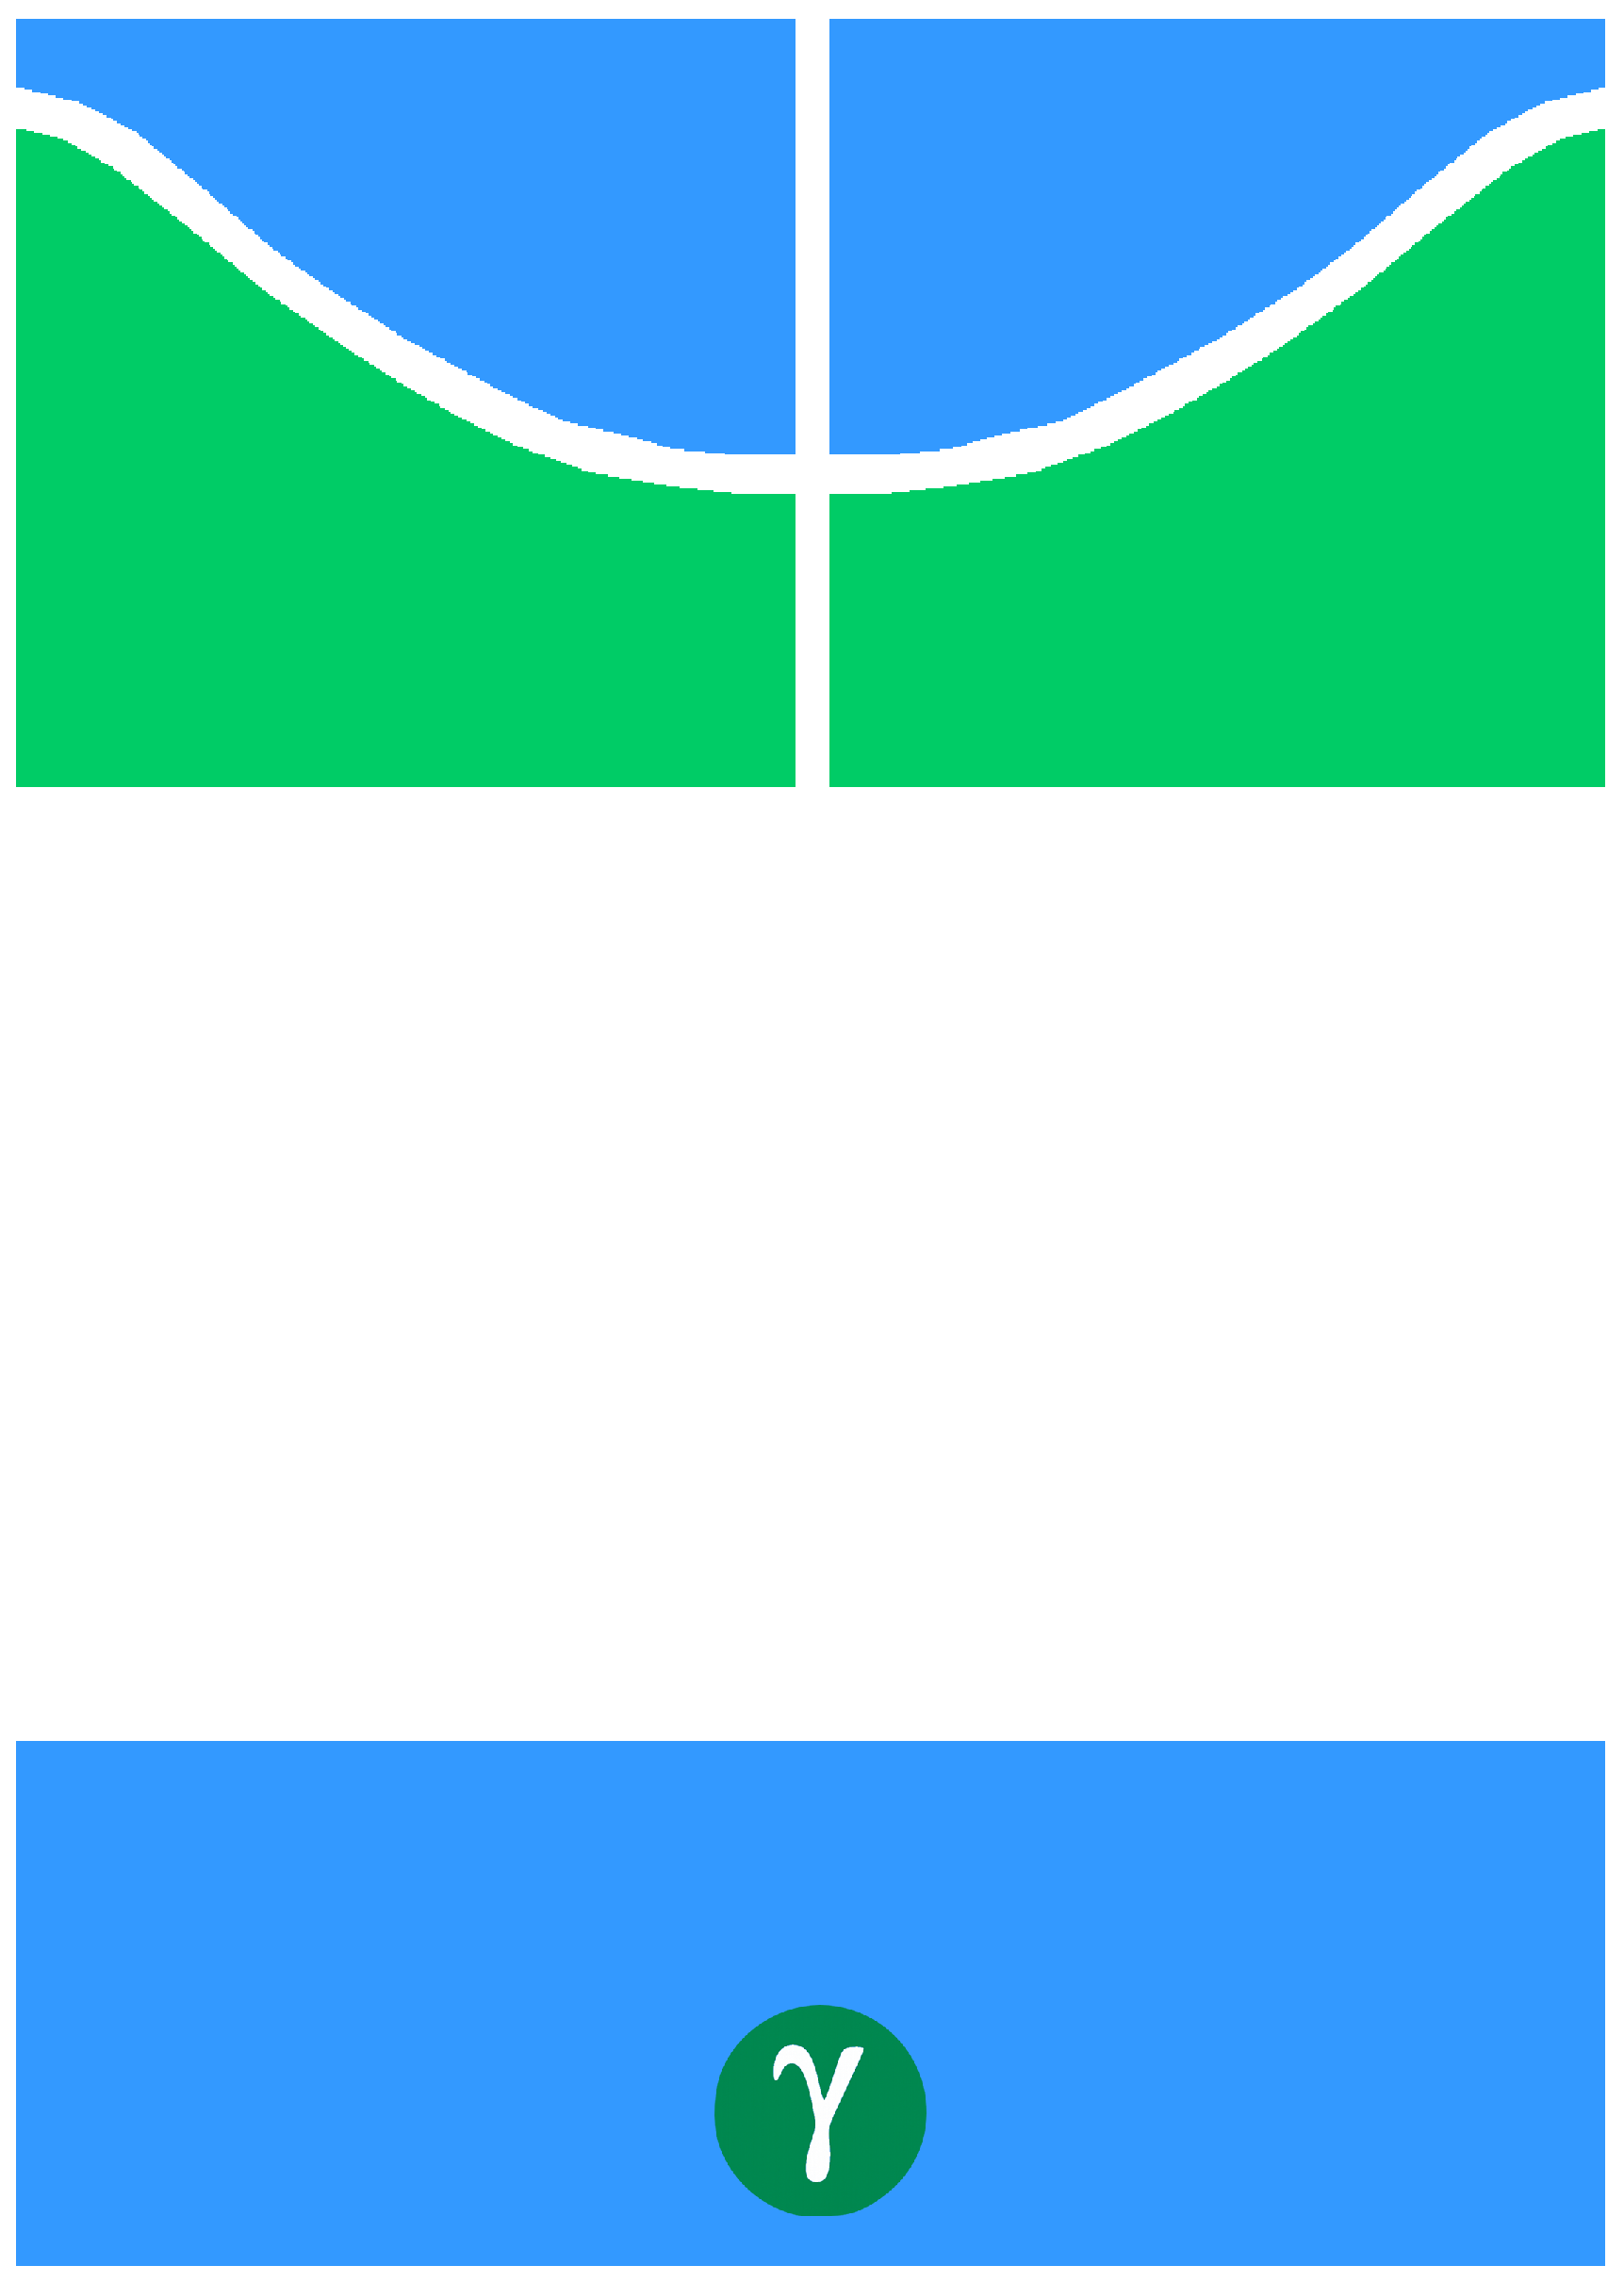
\includegraphics[width=\paperwidth,height=\paperheight,%
				keepaspectratio]{figuras/capa.eps}%
			\vfill
		}
	}
}

\renewcommand{\imprimircapa}{%
  \begin{capa}%
    \center
	\AddToShipoutPicture*{\BackgroundPic}

%	\begin{huge}
%		\textbf{\textsc{Trabalho de Conclusão de Curso}}
%	\end{huge}

    \vspace*{2.7in}
	{\textbf{\large\imprimirinstituicao}}
	\par
	{\textbf{\large\imprimircurso}}

	\vspace{0.5in}

    {\ABNTEXchapterfont\bfseries\LARGE\imprimirtitulo}
    \vspace*{\fill}
    
	\begin{flushright}
    	\textbf{{\large{Autor: \imprimirautor}}}
		\par
    	\textbf{{\large{Orientador: \imprimirorientador}}}
	\end{flushright}
		
    \vspace*{0.2in}
    \textbf{{\large\imprimirlocal}}
    \par
    \textbf{{\large\imprimirdata}}
    
    \vspace*{2.2in}
  \end{capa}
}



% Dados pessoais
\autor{Álvaro Fernando Matos de Souza}
\curso{Engenharia de Software}

% Dados do trabalho
\titulo{Estudo sobre visualização de software aplicado à plataforma web livre Mezuro}
\data{2015}
\palavraChaveUm{Engenharia de Software}
\palavraChaveDois{Visualização de Software}
\palavraChaveTres{Métricas de código-fonte}
\palavraChaveQuatro{Evolução de Software}

% Dados da orientacao
\orientador{Prof. Dr. Paulo Roberto Miranda Meirelles}

% Dados para a ficha catalográfica
\cdu{} 

% Dados da aprovação do trabalho
\dataDaAprovacao{Dezembro de 2015}
\membroConvidadoUm{Rafael Messias Martins}
\membroConvidadoDois{Titulação e Nome do Professor Convidado 02}

\local{Brasília, DF}
\instituicao{%
  Universidade de Brasília - UnB
  \par
  Faculdade UnB Gama - FGA
}
\tipotrabalho{Trabalho de Conclusão de Curso}
\preambulo{Monografia submetida ao curso de graduação em (\imprimircurso) 
da Universidade de Brasília, como requisito parcial para obtenção do Título 
de Bacharel em (\imprimircurso).}

\definecolor{blue}{RGB}{41,5,195}
\makeatletter
\hypersetup{
     	%pagebackref=true,
		pdftitle={\@title}, 
		pdfauthor={\@author},
    	pdfsubject={\imprimirpreambulo},
	    pdfcreator={LaTeX with abnTeX2},
		pdfkeywords={abnt}{latex}{abntex}{abntex2}{trabalho acadêmico}, 
		colorlinks=true,       		% false: boxed links; true: colored links
    	linkcolor=blue,          	% color of internal links
    	citecolor=blue,        		% color of links to bibliography
    	filecolor=magenta,      		% color of file links
		urlcolor=blue,
		bookmarksdepth=4
}
\makeatother
\setlength{\parindent}{1.3cm}
\setlength{\parskip}{0.2cm}  
\makeindex


\begin{document}

\frenchspacing
\imprimircapa
\imprimirfolhaderosto*

\begin{fichacatalografica}
	\vspace*{\fill}					% Posição vertical
	\hrule							% Linha horizontal
	\begin{center}					% Minipage Centralizado
	\begin{minipage}[c]{12.5cm}		% Largura
	
	\imprimirautor
	
	\hspace{0.5cm} \imprimirtitulo  / \imprimirautor. --
	\imprimirlocal, \imprimirdata-
	
	\hspace{0.5cm} \pageref{LastPage} p. : il. (algumas color.) ; 30 cm.\\
	
	\hspace{0.5cm} \imprimirorientadorRotulo~\imprimirorientador\\
	
	\hspace{0.5cm}
	\parbox[t]{\textwidth}{\imprimirtipotrabalho~--~\imprimirinstituicao,
	\imprimirdata.}\\
	
	\hspace{0.5cm}
		1. \imprimirpalavrachaveum.
		2. \imprimirpalavrachavedois.
		3. \imprimirpalavrachavetres.
		4. \imprimirpalavrachavequatro.
		I. \imprimirorientador.
		II. Universidade de Brasília.
		III. Faculdade UnB Gama.
		IV. \imprimirtitulo\\ 			
	
	\hspace{8.75cm} CDU \nomecdu\\
	
	\end{minipage}
	\end{center}
	\hrule
\end{fichacatalografica}

\begin{errata}
Elemento opcional da \citeonline[4.2.1.2]{NBR14724:2011}. \textbf{Caso não 
deseje uma errata, deixar todo este arquivo em branco}. Exemplo:

\vspace{\onelineskip}

FERRIGNO, C. R. A. \textbf{Tratamento de neoplasias ósseas apendiculares com
reimplantação de enxerto ósseo autólogo autoclavado associado ao plasma
rico em plaquetas}: estudo crítico na cirurgia de preservação de membro em
cães. 2011. 128 f. Tese (Livre-Docência) - Faculdade de Medicina Veterinária e
Zootecnia, Universidade de São Paulo, São Paulo, 2011.

\begin{table}[htb]
\center
\footnotesize
\begin{tabular}{|p{1.4cm}|p{1cm}|p{3cm}|p{3cm}|}
  \hline
   \textbf{Folha} & \textbf{Linha}  & \textbf{Onde se lê}  & \textbf{Leia-se}  \\
    \hline
    1 & 10 & auto-conclavo & autoconclavo\\
   \hline
\end{tabular}
\end{table}

\end{errata}

\begin{folhadeaprovacao}

  \begin{center}
    {\ABNTEXchapterfont\large\imprimirautor}

    \vspace*{\fill}\vspace*{\fill}
    {\ABNTEXchapterfont\bfseries\Large\imprimirtitulo}
    \vspace*{\fill}
    
    \hspace{.45\textwidth}
    \begin{minipage}{.5\textwidth}
        \imprimirpreambulo
    \end{minipage}%
    \vspace*{\fill}
   \end{center}
    
   Trabalho aprovado. \imprimirlocal, \imprimirdatadaaprovacao:

   \assinatura{\textbf{\imprimirorientador} \\ Orientador} 
   \assinatura{\textbf{\imprimirmembroconvidadoum} \\ Convidado 1}
   \assinatura{\textbf{\imprimirmembroconvidadodois} \\ Convidado 2}
      
   \begin{center}
    \vspace*{0.5cm}
    {\large\imprimirlocal}
    \par
    {\large\imprimirdata}
    \vspace*{1cm}
  \end{center}
  
\end{folhadeaprovacao}

\begin{agradecimentos}

\textbf{TODO: agradecimentos}.
\end{agradecimentos}

\begin{epigrafe}
    \vspace*{\fill}
	\begin{flushright}
		\textbf{A epígrafe é opcional. Caso não deseje uma, deixe todo
		este arquivo em branco}.

		\textit{``Não vos amoldeis às estruturas deste mundo, \\
		mas transformai-vos pela renovação da mente, \\
		a fim de distinguir qual é a vontade de Deus: \\
		o que é bom, o que Lhe é agradável, o que é perfeito.\\
		(Bíblia Sagrada, Romanos 12, 2)}
	\end{flushright}
\end{epigrafe}

\begin{resumo}
 O Mezuro é uma plataforma \textit{Web} livre de avaliação de código-fonte.
 Considerando que métricas podem ser definidas como medidas de diversas
 características de um software, o Mezuro avalia as métricas estáticas de
 projetos desenvolvidos em certas linguagens. Essas métricas são expostas por
 meio de números e grupos de leituras, expondo ao usuário aspectos de tamanho e
 qualidade do seu projeto, bastando informar apenas a URL do sistema de controle
 de versão remoto.
 O objetivo deste trabalho é realizar uma análise exploratória desta ferramenta,
 abordando aspectos da visualização das métricas de código dos softwares
 analisados por ela.
 São planejadas as seguintes contribuições: validação das configurações de
 métricas do Mezuro e uma especificação de visualização de software.
 Como contribuição científica, ou atividade de pesquisa, será feita a análise
 dos projetos disponibilizados no Portal do Software Público Brasileiro (SPB)
 escolhidos pois há possibilidade de incorporação do Mezuro neste Portal. Além
 do envolvimento do aluno em parte da evolução do SPB.
 Outra contribuição será a realização do estudo das possíveis técnicas de
 visualização de software aplicadas ao Mezuro.

 \vspace{\onelineskip}

 \noindent
 \textbf{Palavras-chaves}: Engenharia de Software. Mezuro.
 Métricas de código-fonte. Evolução de Software. Visualização de Software.
 Software Público Brasileiro.
\end{resumo}

\begin{resumo}[Abstract]
 \begin{otherlanguage*}{english}
   This is the english abstract.

   \vspace{\onelineskip}
 
   \noindent 
   \textbf{Key-words}: latex. abntex. text editoration.
 \end{otherlanguage*}
\end{resumo}

\pdfbookmark[0]{\listfigurename}{lof}
\listoffigures*
\cleardoublepage
\pdfbookmark[0]{\listtablename}{lot}
\listoftables*
\cleardoublepage

\begin{siglas}
  \item[VS] Visualização de Software
  \item[URL] Uniform Resource Locator - Localizador Padrão de Recursos
  \item[CLI] Command-line interface - Interface de linha de comandos
  \item[PHPMD] PHP Mess Detector - Detector de Desordem em Códigos PHP
\end{siglas}

\pdfbookmark[0]{\contentsname}{toc}
\tableofcontents*
\cleardoublepage


\textual

\chapter{Introdução}

% Primeiros parágrafos devem conter de forma clara o que o autor pretende com
% relação aos aspectos científicos e técnicos.

Aspectos da qualidade não são claros em muitos softwares atualmente e existe
uma grande complexidade em entender o seu funcionamento. A visualização de
software pode auxiliar e ou facilitar o entendimento destes aspectos e pode
reduzir essa complexidade. Não faltam dados disponíveis publicamente para
auxiliar na geração desse entendimento: código-fonte, históricos de evolução do
repositório, conjuntos de testes, relatórios de erros e suas soluções, trocas
de mensagens entre membros do projeto em listas de e-mail, artigos escritos por
acadêmicos que buscam fama, entre outros \cite{messias2012}
\cite{benkler2006wealth}.

É preciso processar esses dados de forma correta. E considerando também que,
desenvolvedores são cruciais para o sucesso de um projeto e os valores
numéricos dos vários locais com dados disponibilizados publicamente em que é
possível coletar os dados citados no parágrafo anterior, as vezes podem não ter
uma boa apresentação. Os dados podem ser de pouco valor, pois são numerosos e
difíceis de avaliar. Uma possível solução: visualização de informação
\cite{messias2012}. Visualizações de informação são ``representações visuais e
interativas de dados, apoiadas por computador, utilizadas para amplificar a
aquisição de conhecimento e apoiar descobertas, tomadas de decisão e
explicações a partir de dados complexos'' \cite{card1999readings}. Um problema
da visualização de software é selecionar uma técnica, pois nenhuma técnica
específica funciona para todos os problemas.

O software livre apresenta certas vantagens em detrimento ao software restrito.
Geralmente licenciado sob as definições da
\textit{Free Software Foundation}\footnote{\url{http://www.gnu.org/philosophy/free-sw.pt-br.html}},
ou da \textit{Open Source Initiative}\footnote{\url{https://opensource.org/docs/definition.html}},
o software livre e aberto (\textit{Free and Open Source Software} - FOSS) tem
seu código aberto e acessível ao público e garante ao programador certos
aspectos que podem simplificar o desenvolvimento de um novo software ou a
evolução de um outro onde o envolvimento é desejado, seja por questões de
melhoria, éticas, personalização ou simplesmente pelo interesse pessoal
\cite{meirelles2013monitoramento}. E muitas outras características agregam
valor ao uso, desenvolvimento e estímulo às contribuições ao FOSS: o
estabelecimento de uma \textit{cultura livre}, valorizando o mérito de questões
técnicas inerentes ao desenvolvedor; reconhecimento de bons programadores
capazes de escreve bom código e outros programadores melhores ainda capazes de
mantê-lo; reconhecimento do valor das pessoas envolvidas e interessadas, sejam
usuários finais ou testadores de versões instáveis de software; entre outras
características \cite{raymond1999cathedral}.

Metodologias ágeis estão fortemente ligadas ao desenvolvimento de FOSS e
possuem formas de trabalho semelhantes \cite{meirelles2013monitoramento}. Esse
vínculo é expresso majoritariamente pelos os valores \cite{beck2001manifesto}:

\begin{itemize}
  \item Indivíduos e interações são mais importantes que processos e
  ferramentas;
  \item Software em funcionamento é mais importante que documentação abrangente;
  \item Colaboração com o cliente (usuários) é mais importante que negociação
  de contratos;
  \item Responder às mudanças é mais importante que seguir um plano.
\end{itemize}

Métricas de código estão ligadas ao desenvolvimento, planejamento, custos,
produtividade e qualidade do software. Existem dois grandes conjuntos delas:
métricas tradicionais e métricas de orientação a objetos. São métricas
tradicionais: métricas de tamanho (ex. Linhas de Código - LOC), métricas de
complexidade (ex. Complexidade Ciclomática), métricas manutenibilidade, dentre
outras (Tamanho Médio dos Módulos, Uso de Variável, Número de Funções, por
exemplo). E são métricas de orientação a objetos: métricas de classes (ex.
Encapsulamento dos Atributos), métricas de métodos (ex. Média de Complexidade
dos Métodos), métricas de acoplamento (ex. Acoplamento Aferente), métricas de
herança (ex. Medida de Polimorfismo) e métricas de sistema (ex. Reúso de
Classe) \cite{meirelles2013monitoramento}.

% Introdução com forte embasamento em Métodos Ágeis e FOSS, e Visualização pra apoiar
% citar PRMM, Fábio Kon... (verificar referências do Messias)

\section{Contexto}

Neste trabalho de conclusão de curso são apresentadas as relações entre
visualização de software, FOSS e metodologias ágeis com as devidas adaptações e
métricas de código-fonte para observação de que o entendimento do software e a
averiguação da qualidade do mesmo são passiveis através da visualização de
software. Para tanto, é proposto a adequação de técnicas usualmente utilizadas
para a geração de visualizações da informação às ferramentas de monitoramento
estático de código-fonte, em especial ao
Mezuro\footnote{\url{http://mezuro.org/}}.

\section{Objetivos}

Inicialmente a proposta deste trabalho é a geração de visualizações que podem
ser \textit{instanciadas} em determinadas ferramentas de monitoramento de
código-fonte, dada as adaptações para a coleta dos resultados da mesma. Com o
foco no Mezuro, o objetivo deste trabalho é investigar e utilizar-se da
visualização de software para auxiliar o controle da qualidade de um software.
É feito a união de determinadas métricas para gerar uma ou várias visualizações
que auxiliem o usuário a ter uma melhor interpretação do resultado gerado por
esta ferramenta.

\section{Organização do Trabalho}

O trabalho está organizado da seguinte maneira: Capítulo 2, onde será tratada a
VS como principal base para o referencial teórico e revisão bibliográfica;
Capítulo 3, que trata da metodologia para o desenvolvimento do mesmo; no
Capítulo 4 são apresentados os resultados preliminares com explicação do
principal exemplo de uso; e o Capítulo 5 com as conclusões, trabalhos futuros e
cronograma de atividades.

% Introdução com forte embasamento em Métodos Ágeis e FOSS, e Visualização pra apoiar
% citar PRMM, Fábio Kon... (verificar refereências do Messias)
\chapter{Visualização de Software}

\textit{``Imagination or visualization, and in particular the use of diagrams,
has a crucial part to play in scientific research.''} René Descartes, 1637.

Há muito informação hoje disponível, circulando e com um fluxo de crescimento
exponencial. Grande parte dessa informação é útil para o ensino e a instrução.
Dados são recursos valiosos, porém é preciso compreendê-los \cite{messias2012}.

A visualização de um dado com propriedades visuais como posição, tamanho, forma
e cor, potencializam as habilidades sensoriais do homem. Possivelmente o usuário
irá extrair observações e conclusões sobre os dados, e também poderá moldar esse
conhecimento adquirido para atingir os objetivos \cite{card1999readings}
\cite{heer2012interactive} \cite{keim2002information}.

O estudo da visualização pode ser dividido em duas grandes vertentes, ambas
possuindo interação com usuário induzindo-o ao entendimento das informações
contidas nos dados \cite{de2003visual}:

\begin{enumerate}
  \item \textbf{Visualização Científica}: dados físicos e inerentemente
  geométricos;
  \item \textbf{Visualização de Informação}: informações não físicas, por
  exemplo coleções de documentos, podem ser beneficiadas, porém não há nenhuma
  forma óbvia de se mapear tais dados em uma imagem \cite{card1999readings}.
  Envolve algo mais complexo.
\end{enumerate}

Visualização da informação é por tanto relacionada a \textbf{grandes conjuntos}
de dados. Um \textbf{conjunto} é um o número de atributos ou dimensões que o
identifica. Quantidade de dimensões é o mesmo que \textbf{dimensionalidade}.

Os tipos de dados comuns são: bidimensionais e multidimensionais
\cite{de2003visual}.

Os multidimensionais necessitam da aplicação de uma técnica
\cite{keim2002information}. São técnicas citadas por \citeonline{messias2012}:

\begin{itemize}
  \item Projeções geométricas:
	\begin{itemize}
		\item Coordenadas paralelas. Exemplo na Figura \ref{fig:parallel};
	\end{itemize}
  \item Orientadas a pixel:
	\begin{itemize}
		\item \textit{recursive patterns};
		\item \textit{circle segments};
	\end{itemize}
  \item Iconográficas:
	\begin{itemize}
		\item \textit{stick figures};
	\end{itemize}
  \item Hierárquicas:
	\begin{itemize}
		\item \textit{Dimensional Stacking}.
	\end{itemize}
\end{itemize}

\begin{figure}[!htb]
  \centering
    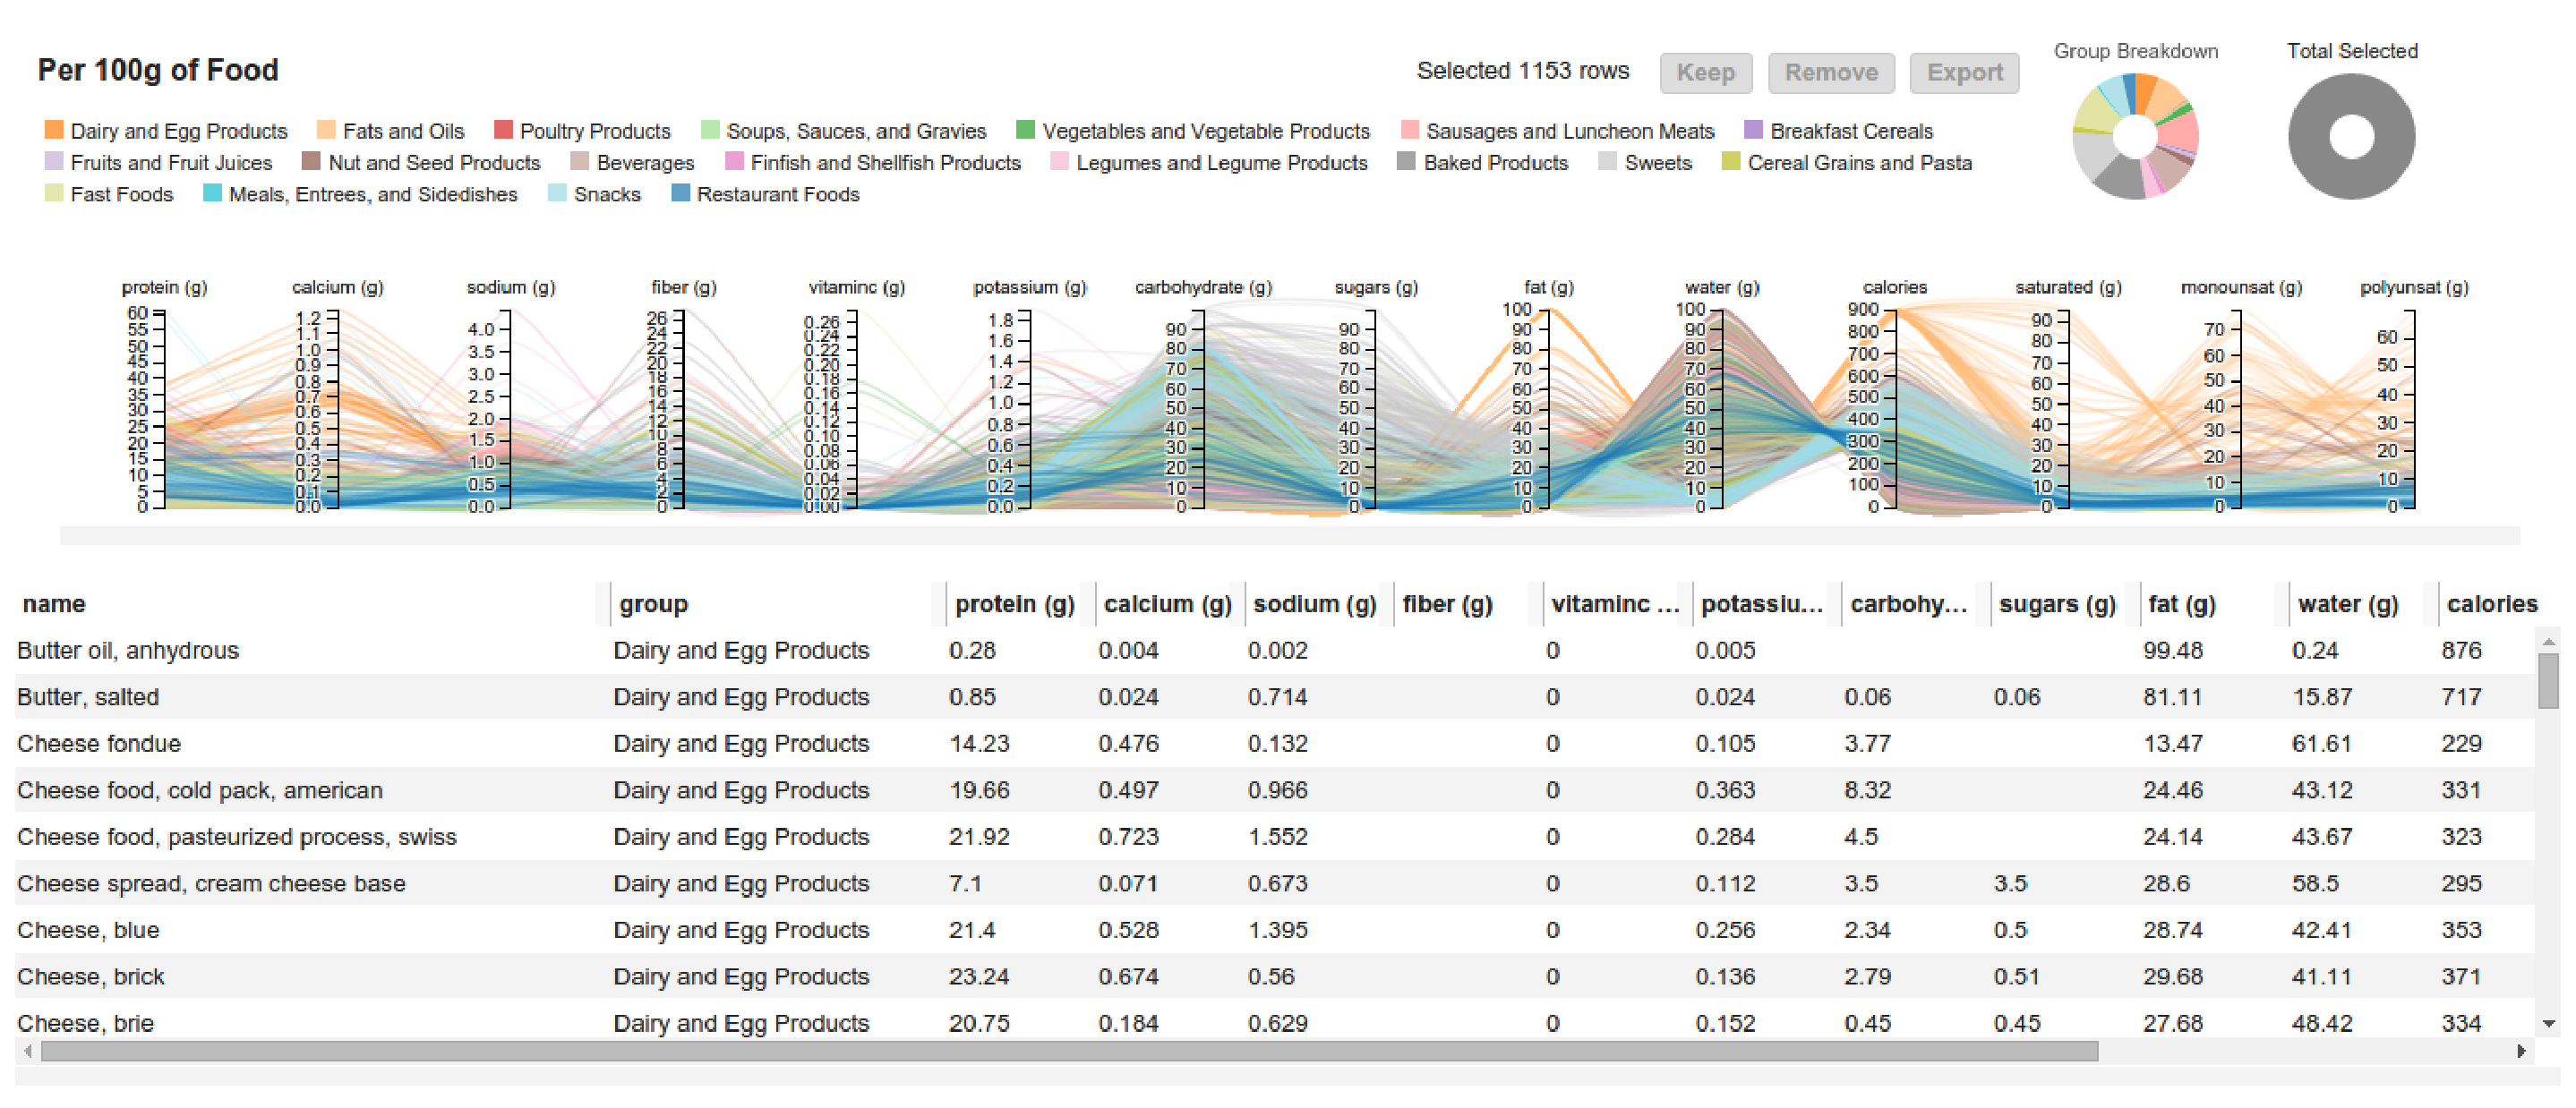
\includegraphics[keepaspectratio=true,scale=0.3]
    {figuras/parallel.eps}
  \caption{Exemplo de Coordenadas Paralelas \cite{kaichang2015}}
  \label{fig:parallel}
\end{figure}

Por tanto, segundo \citeonline{diehl2007software}, Visualização de Software (VS)
é uma subárea da Visualização de Informação. E os objetivos dela são: ``auxiliar
a compreensão de sistemas complexos de software e melhorar a produtividade do
processo de desenvolvimento'' \cite{messias2012}. É a representação gráfica de
aspectos técnicos, ou sociais, ou ambos de um software. As técnicas geram
exibições de aspectos do software que podem auxiliar tarefas de:

\begin{itemize}
	\item Gerenciamento;
	\item Projeto;
	\item Implementação;
	\item Depuração;
	\item Análise;
	\item Manutenção.
\end{itemize}

Visualização de Software é um dos braços da Visualização de Informação que mais
cresce \cite{telea2014data}. \citeonline{bassi2001software} apresentam alguns
benefícios de se utilizar ferramentas de VS:

\begin{itemize}
	\item Economia de tempo e dinheiro;
	\item Melhor compreensão;
	\item Aumento da produtividade;
	\item Auxílio na detecção de erros no código;
	\item Melhoria da qualidade.
\end{itemize}

\section{Categorias da Visualização de Software}

A visualização de software pode ser levada em consideração pelas três seguintes
categorias: estrutura, comportamento e evolução \cite{diehl2007software}.

\subsection{Estrutura}

Relacionada ao que é estático em um software, sem necessidade de executá-lo. Por
exemplo: o código-fonte, as estruturas de dados do programa, o grafo de chamadas
estático e a organização do sistema em módulos \cite{diehl2007software}.

Propriedades interessantes \cite{messias2012}:

\begin{itemize}
	\item Exatidão: linguagens de programação exacerbadamente definidas;
	\item Grande escala: sistemas que possuem uma quantidade grande de linhas
	de código;
	\item Relações e hierarquias entre entidades do código;
	\item Diversos atributos que expressam as características dessas entidades.
\end{itemize}

Ferramentas de geração de visualização da categoria estrutura compartilham o
mesmo modelo conceitual: a geração de um grafo que relaciona em seus vértices
as propriedades anteriormente citadas.

Exemplos de Visualização da estrutura de software: \textit{Team Assessment}
\cite{telea2009case} e \textit{CodeCity} \cite{wettel2008codecity}.

Uma técnica bastante elaborada, desenvolvida por \citeonline{holten2006hierarchical},
expressa em uma única imagem duas das propriedades: a estrutura hierárquica e
suas dependências internas (Figura \ref{fig:heb}).

\begin{figure}[!htb]
  \centering
    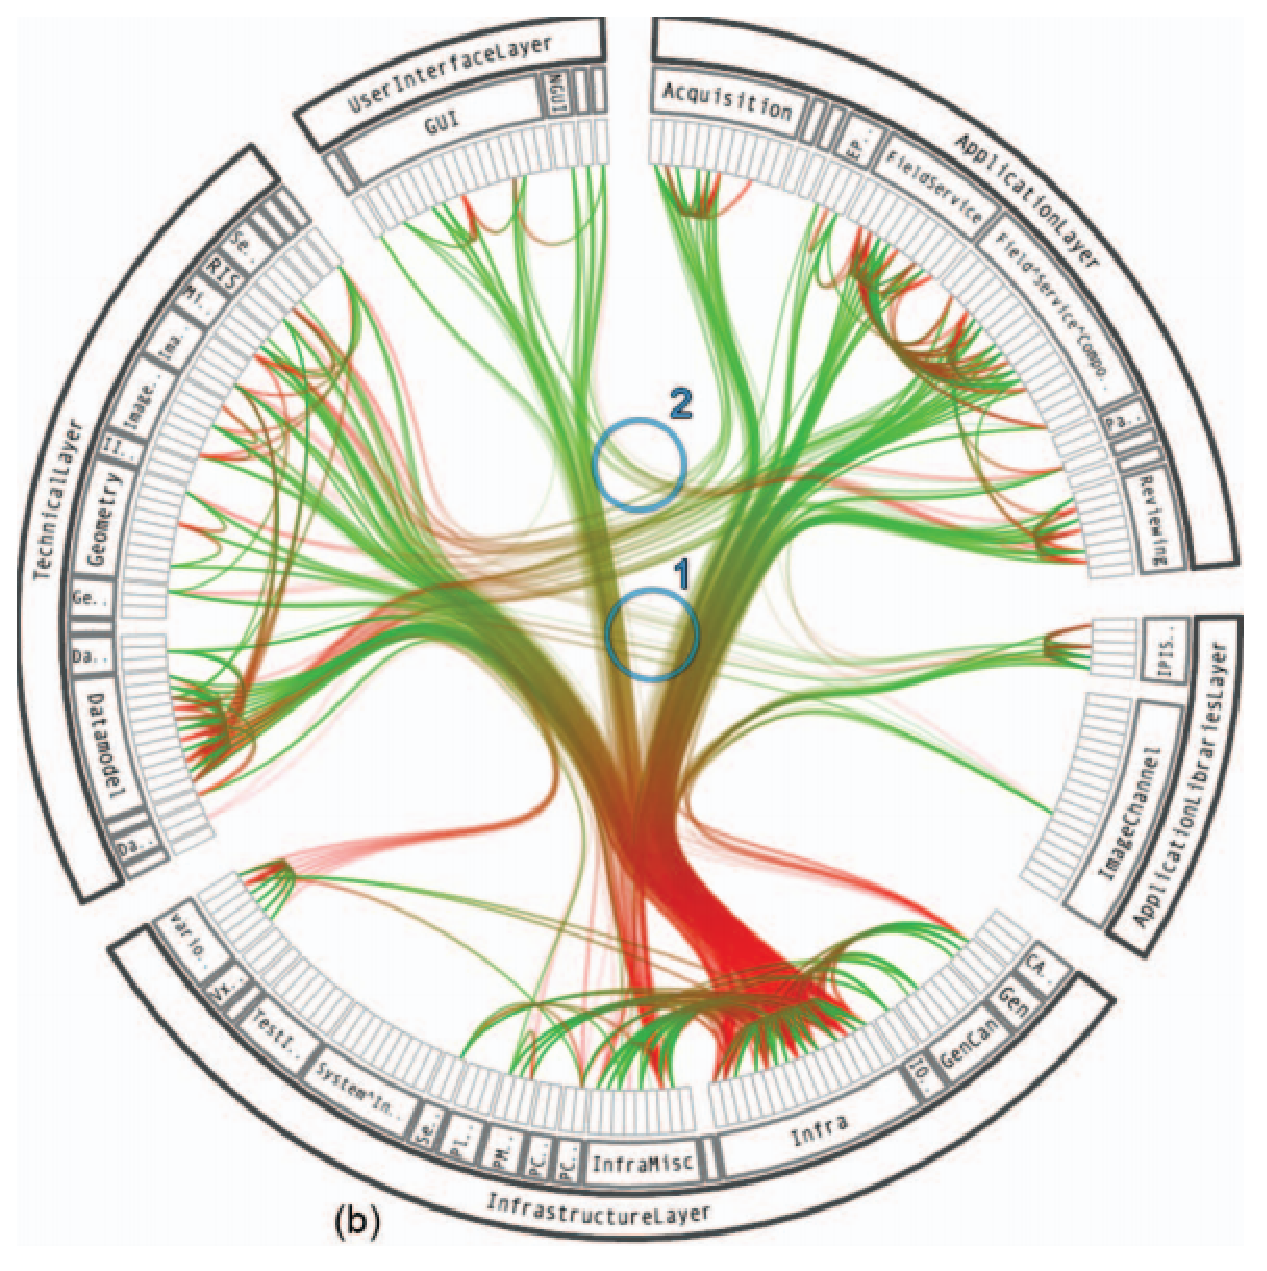
\includegraphics[keepaspectratio=true,scale=0.5]
    {figuras/heb.eps}
  \caption{Estrutura Hierárquica \cite{holten2006hierarchical}}
  \label{fig:heb}
\end{figure}

Métricas podem ser incluídas em visualizações da estrutura. Na ferramenta
SolidSX (Figura \ref{fig:solidSX}), \citeonline{reniers2011visual} inclui
algumas métricas como linhas de código, comentários e complexidade. Essa
ferramenta une três técnicas:

\begin{itemize}
	\item \textit{TreeMap} - disposição das hierarquias do código;
	\item \textit{HEB};
	\item \textit{TableLens} - módulos são linhas e métricas são colunas de uma
	tabela, mapeando as métricas e destacando-as por cores.
\end{itemize}

\begin{figure}[!htb]
  \centering
    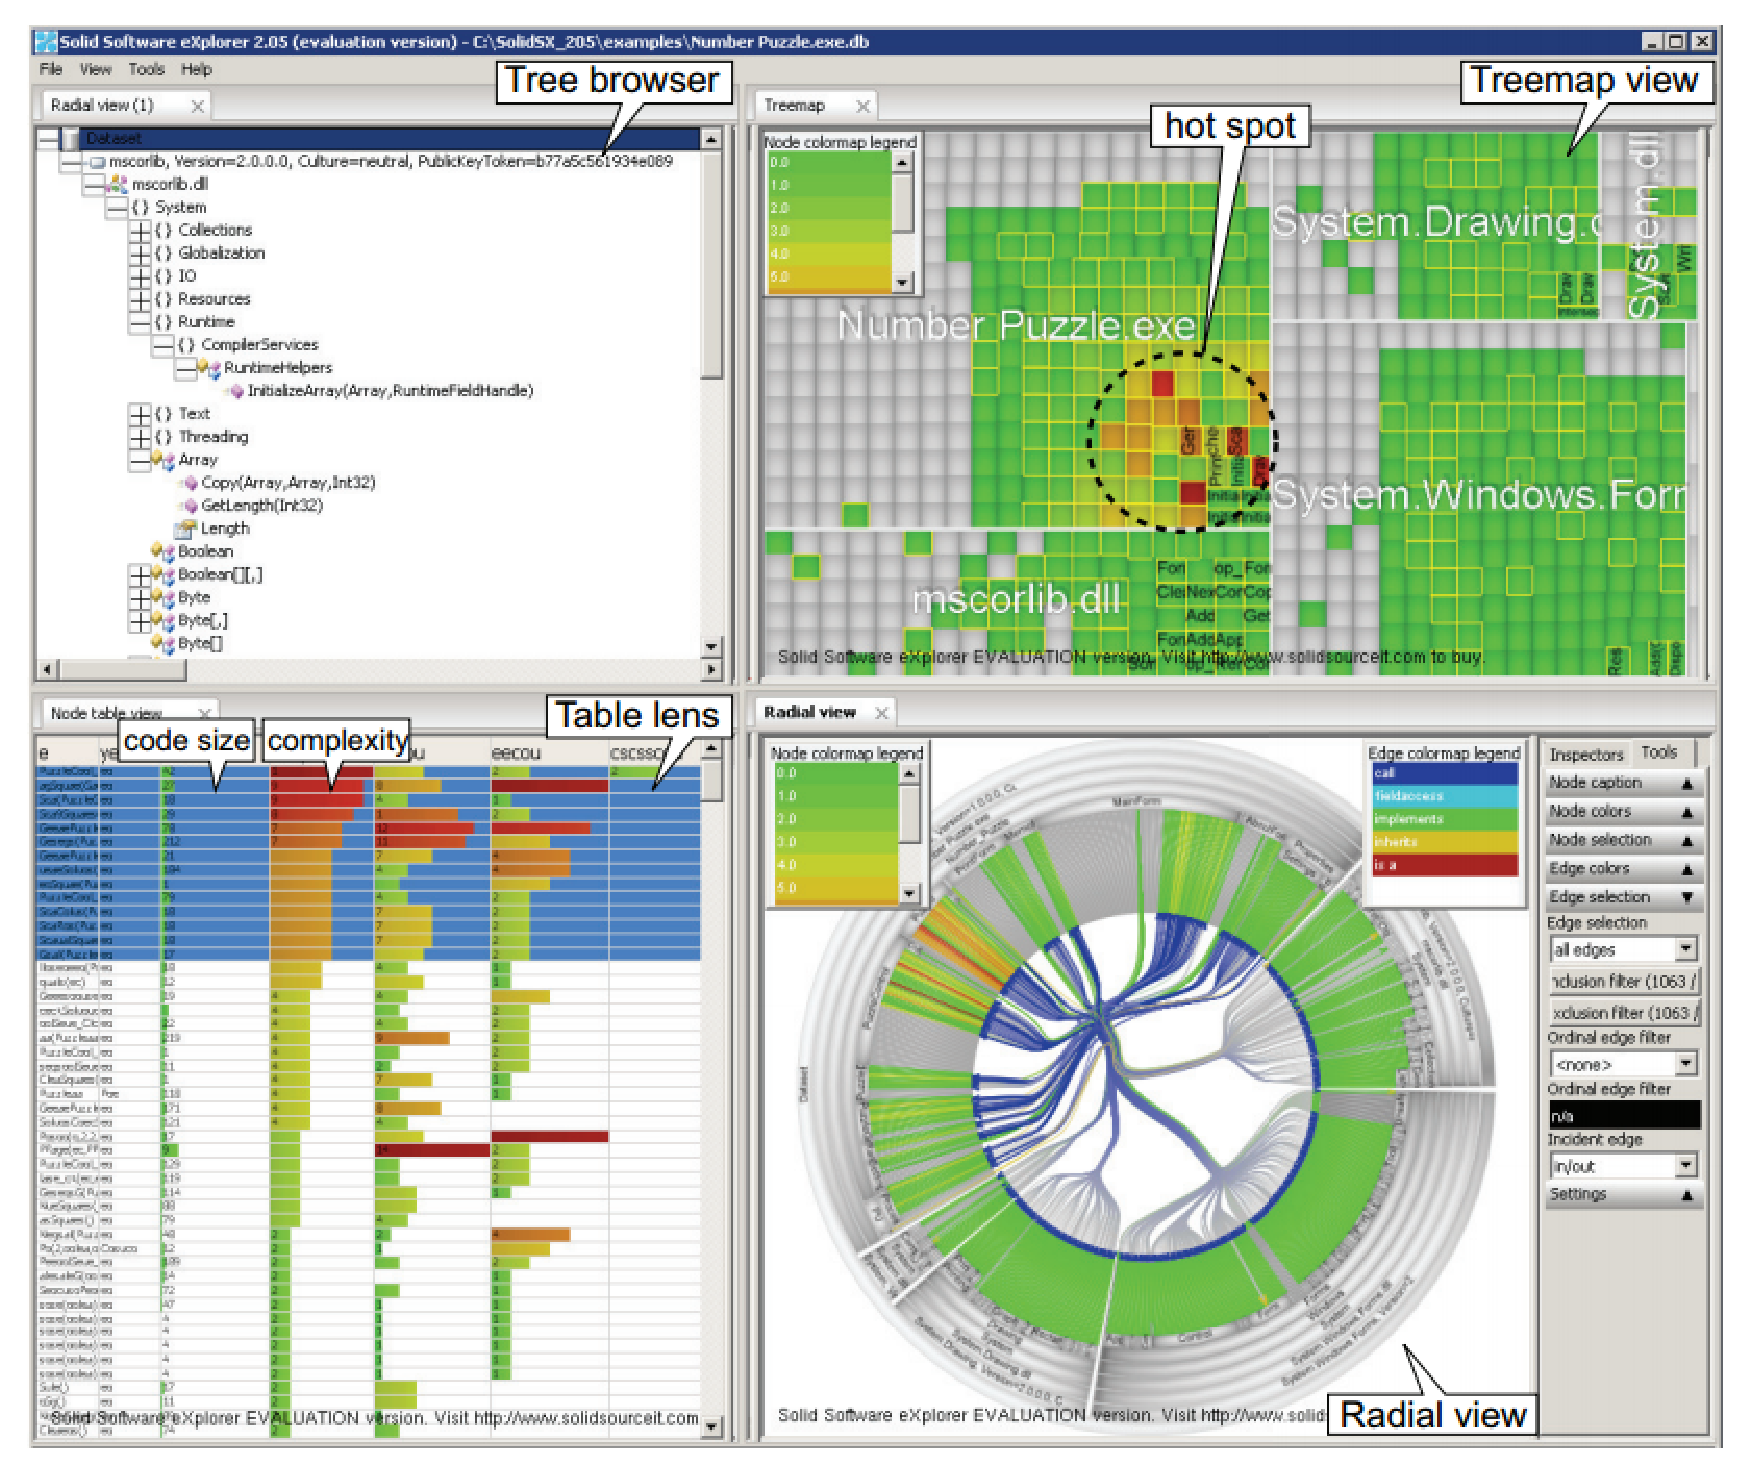
\includegraphics[keepaspectratio=true,scale=0.5]
    {figuras/solidSX.eps}
  \caption{Ferramenta SolidSX \cite{reniers2011visual}}
  \label{fig:solidSX}
\end{figure}

\subsection{Comportamento}

O software é executado. Análise do que acontece, em tempo de execução, dada
determinada entrada. Técnica: sequência de estado. Combinar dados e código para
analisar interação com a memória. Dependendo do paradigma de programação, pode
haver uma relação entre os métodos ou funções e a comunicação entre os objetos
\cite{cornelissen2009systematic} \cite{diehl2007software}.

Aplicações dessa categoria:

\begin{itemize}
	\item Análise de traces de execução;
	\item Visualização dinâmica e recuperação de arquitetura;
	\item Animação de algoritmos;
	\item Depuração visual;
	\item Poio visual à atividade de teste.
\end{itemize}

Exemplo da ferramenta \textit{Tarantula} \cite{jones2002visualization} -
Depuração visual, execução de testes, destaque com escala que vai de vermelho
(falha) até verde (sucesso).

\subsection{Evolução}

Categoria aplicada para compreensão das modificações ao longo do tempo. A
manutenção e evolução de um sistema pode chegar a 80\% do custo total de
desenvolvimento \cite{pfleeger2005analyzing}. Dado este que fortalece as
visualizações desta categoria.

\citeonline{biggerstaff1993concept} dizem que: ``Uma pessoa entende um programa
quando ele ou ela é capaz de explicar o programa, a estrutura, o seu
comportamento, os efeitos no seu contexto operacional, e os seus relacionamentos
com o domínio da aplicação em termos que são qualitativamente diferentes dos
\textit{tokens} usados para a construção do código-fonte do programa.'' Essa
definição de entendimento se alinha com as duas primeiras categorias do estudo
de visualização, e entender a evolução de software pode ser igualmente
importante como entender sua estrutura, considerando aspectos gerenciais e
administrativos também.

% TODO: INICIAR COM O CAPÍTULO 2 SOBRE VISUALIZAÇÃO
% capitulo 2 - visualização - com seção de métricas
% msg pro leitor: explicar visu, oq ele precisa saber para ler o meu TCC
\chapter{Metodologia}

\section{Objetivos}

O objetivo deste capítulo é apresentar a metodologia utilizada para a
realização da pesquisa e contribuição tecnológica. A principal questão
a ser respondida é: como a visualização de software pode auxiliar na
interpretação das métricas coletas e calculadas por ferramentas de análise
de código?

Considerando esta questão, é importante ressaltar que existem incontáveis
destas ferramentas. Porém estas analisam apenas aspectos mui específicos
do software, e falham (algumas delas) em demostrar ao engenheiro de
qualidade a interpretação dos dados analisados \cite{deissenboeck2011}.

Neste trabalho serão unidas determinadas métricas (TODO: definir quais
métricas), para gerar uma ou várias visualizações que auxiliem o usuário
do Mezuro a ter uma melhor interpretação do resultado gerado por esta
ferramenta.

Como exemplo dessa união e para a construção do exemple de uso, é proposto
utilizar-se da decisão dos colegas Renan Costa Filgueiras e Vinícius Vieira
Meneses: foram escolhidas três métricas para a configuração da visualização em
radar: \textit{number of methods} (código: npm), \textit{number of public
methods} (código nom) e \textit{total number of modules} (código:
total\_modules); e a decisão de utilizar a biblioteca Javascript \textit{D3.js -
Data-Driven Documents} \cite{filgueiras2014mezuro}.

\section{Trabalhos Relacionados}

\section{Questão Problema e Hipóteses}

Reforçando a questão problema (QP), foram levantadas estas outras abaixo:

\begin{itemize}
  \item QP1 - Como a visualização de software pode auxiliar na
  interpretação das métricas coletadas e calculadas pelo Mezuro?
  \item QP2 - Quais técnicas de visualização que melhor se adequam ao
  contexto do Mezuro, possibilitando a aplicação em qualquer contexto de
  configuração?
  \item QP3 - Como representar as diferentes perspectivas sobre o processo
  de desenvolvimento e o produto de software?
\end{itemize}

As hipóteses são:

\begin{itemize}
  \item H1 - Não haverá uma visualização única para todas as métricas.
  \item H2 - Algumas métricas poderão ser apresentadas de uma forma combinada
  em uma única representação/visualização.
\end{itemize}

% TODO: elaborar e documentar as hipótees

\section{O Mezuro}

O projeto Mezuro é uma ferramenta para extração, análise e interpretação de
métricas de código-fonte. De uma forma geral, ele é dividido em duas partes:
para o processamento e para o cálculo é utilizado o Kalibro, que é um
\textit{webservice}; e o Prezento para a interface gráfica (uma aplicação
\textit{Web}) \cite{meirellesCibse2015}. Sob a licença
\textit{Affero General Public License version 3} (AGPLv3), o Mezuro permite que
o usuário crie, salve e edite ``configurações'' que são um conjunto de
métricas escolhidas por este e um ``grupo de leitura'' para provimento de uma
interface gráfica de um conjunto de leitura que tenha algum sentido quando
agrupadas, por exemplo: com a pontuação x, a métrica terá o ``rótulo'' ``BOM'' e
será atribuído à ela a cor amarela; com a pontuação x + 2, a métrica terá o
``rótulo'' ``ÓTIMO'' e estará com a cor verde. As cores são para destacar a
interpretação e são definidas com valores hexadecimal \cite{camarinhaOSS2015}.

O Kalibro, citado no parágrafo anterior, foi inicialmente escrito em Java para
compor uma das ferramentas do projeto QualiPSo (\textit{Quality Platform for
Open Source Software}). Já possuía maioria das funcionalidades presentes na
versão atual do Mezuro. Uma delas, bastante prática, é a de fornecer apenas o
URL do código compactado em arquivo ZIP ou TARBALL, ou o link para as
aplicações de controle de versão em SVN ou GIT, mais a escolha de uma
configuração, para iniciar a análise \cite{camarinhaOSS2015}. Em 2013 o Mezuro
passou a ser reescrito em Ruby, com objetivo de manter na mesma tecnologia as
camadas da arquitetura. Mudança justificada também pela necessidade do
processamento dos cálculos e da análise. A carga de requisições, mais a
quantidade de núcleos que o servidor possuía, faziam com que a versão original
do Kalibro ficasse debilitado em seu fluxo de execuções. Outra vantagem dessa
reescrita é a facilidade com que novos contribuidores puderam/poderão entender
todo o funcionamento dessa parte do Mezuro. Algumas funcionalidades foram
eliminadas por serem consideradas não essenciais. E grande parte da primeira
versão do Kalibro está presente na gema
kalibro\_gem\footnote{\url{https://rubygems.org/gems/kalibro_gem}}
\cite{meirellesCibse2015}.

% TODO: a gem kalibro\_gem e a kalibro\_client são a mesma coisa? A kalibro\_gem
% foi descontinuada?)

% Sobre o Prezento

O Kalibro foi construído, nos primórdios, como um plugin da rede social
Noosfero. Com a decisão de reescrevê-lo em Ruby, a antiga interface gráfica,
que era aproveitada do Noosfero, foi também reescrita nesta
tecnologia. O Prezento, desenvolvido utilizando o \textit{framework} para
desenvolvimento de aplicações \textit{Web}
Ruby on Rails\footnote{\url{http://guides.rubyonrails.org/getting_started.html}},
é a redesenha e atual interface.

% Sobre a arquitetura do Mezuro

% (Eu preciso falar do QualiPSo?  Não!)

O projeto QualiPSo, iniciado em meados de 2007, tinha como objetivo aprimorar
as práticas de desenvolvimento aberto à época para atingir o reconhecimento e
confiabilidade que o FOSS possui hoje \cite{messias2012}.

\subsection{Arquitetura e principais funcionalidades do Mezuro}

Com a reescrita, a arquitetura do Mezuro foi dividida em três serviços:

\begin{itemize}
  \item Prezento: para a interface gráfica do usuário
  \item Kalibro Processor: para a análise do código
  \item Kalibro Configurations: para o gerenciamento das configurações
\end{itemize}

A decisão de dividir o Kalibro em serviços separados foi tomada para deixar
cada um deles com menos responsabilidades, facilitando a manutenção e evolução
\cite{camarinhaOSS2015}. E a comunicação entre estes serviços é feita através
do Kalibro Client: um quarto software também escrito em Ruby, mantendo a
escolha de centralização em uma única tecnologia. E para simplificar a
implementação, também foi decidido que a comunicação entre os serviços seria
RESTful.

As figuras a seguir demonstram como a comunicação funciona, um diagrama UML de
sequência do processo de criação de uma configuração chegando ao estágio em que
são expostos os resultados finais de uma análise após a reescrita da interface
gráfica, e outra que demonstra o estado atual do projeto.

\begin{figure}[!htb]
	\centering
    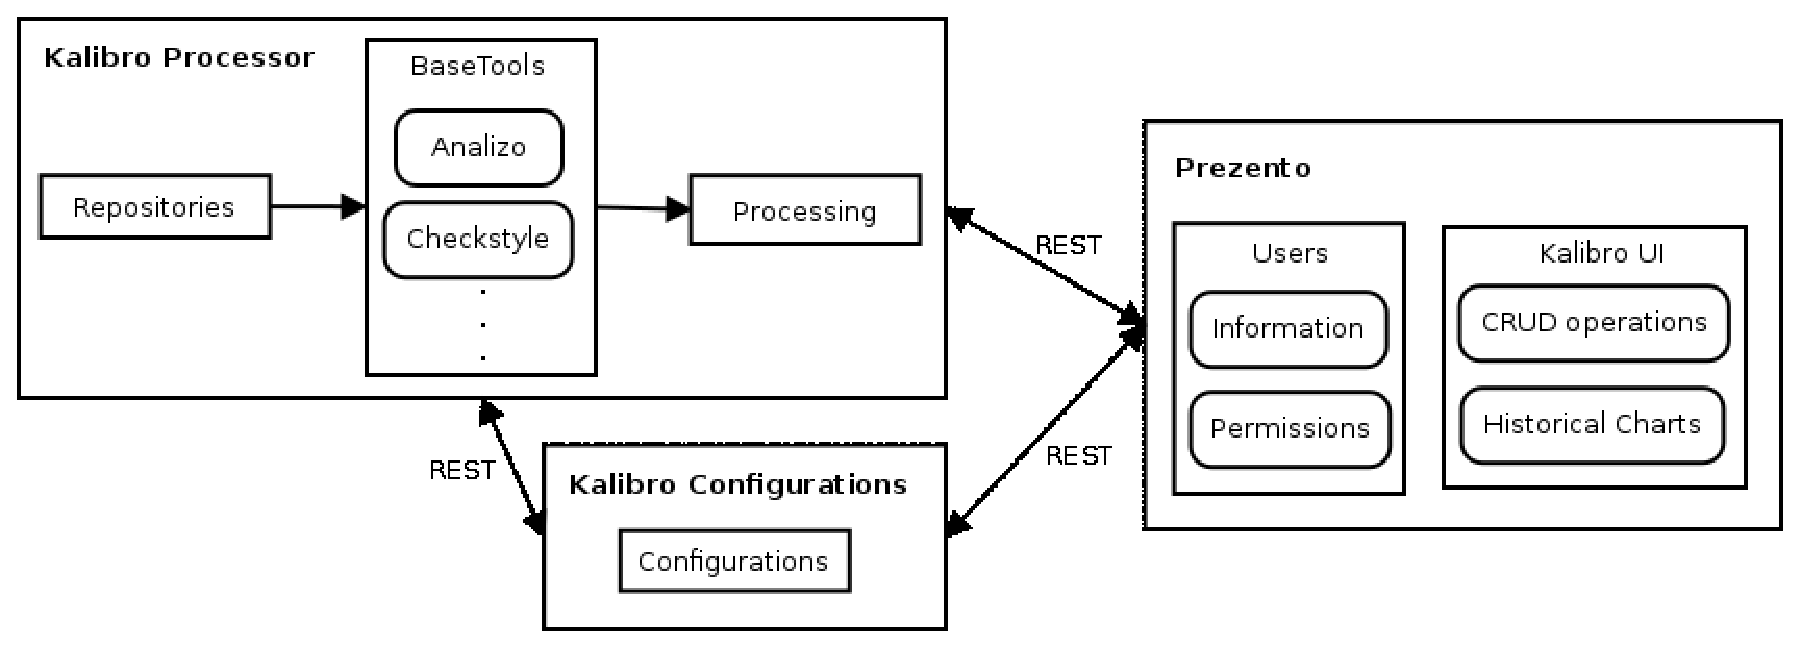
\includegraphics[keepaspectratio=true,scale=0.5]
    {figuras/mezuroCloudArch.eps}
  \caption{Arquitetura do Mezuro \cite{camarinhaOSS2015}}
	\label{fig:mezuroNoosferoArch}
\end{figure}

\begin{figure}[!htb]
	\centering
    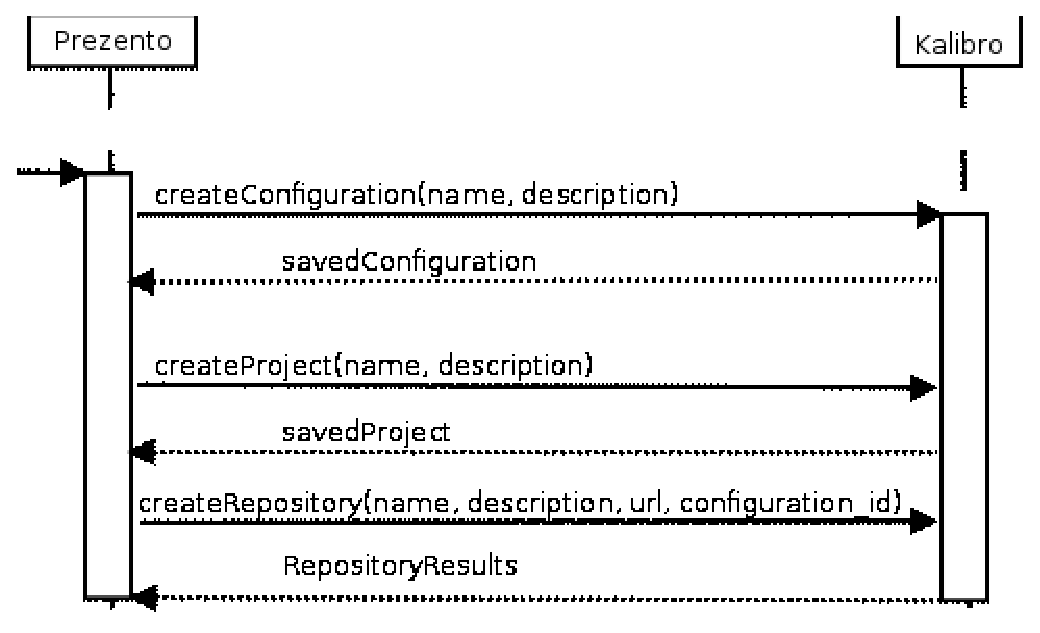
\includegraphics[keepaspectratio=true,scale=0.7]
    {figuras/prevProcessingSeqDiag.eps}
  \caption{Arquitetura do sistema ao fim da reescrita da interface gráfica
  \cite{meirellesCibse2015}}
	\label{fig:prevProcessingSeqDiag}
\end{figure}

\begin{figure}[!htb]
	\centering
    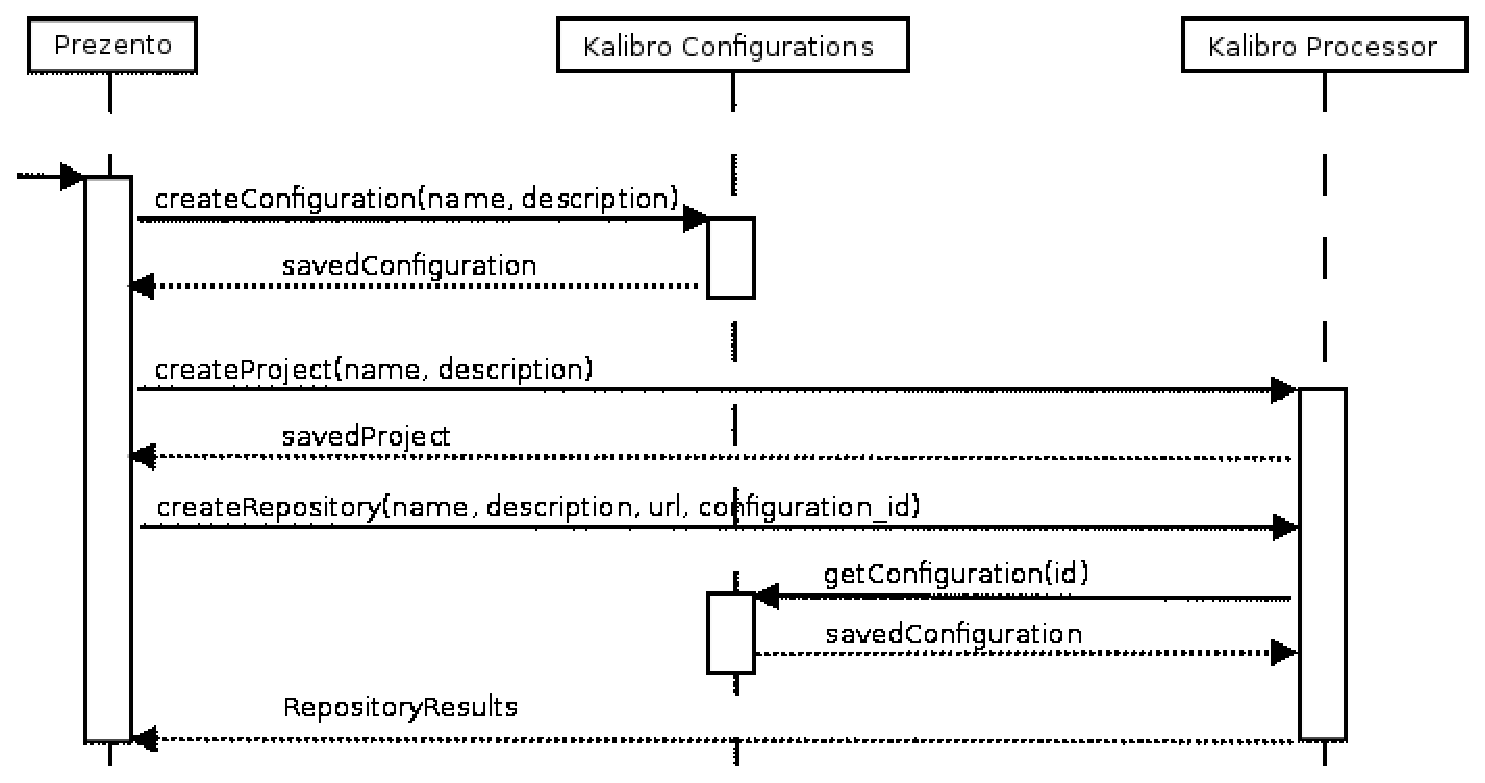
\includegraphics[keepaspectratio=true,scale=0.5]
    {figuras/processingSeqDiag.eps}
  \caption{Arquitetura do sistema ao fim da reestruturação do Kalibro
  \cite{meirellesCibse2015}}
	\label{fig:processingSeqDiag}
\end{figure}

\newpage

Segundo \citeonline{camarinhaOSS2015}, as principais ``funcionalidades podem ser
divididas em dois grupos:

\begin{itemize}
  \item Projeto
    \begin{itemize}
    \item \textit{Download} do código-fonte a partir de repositórios (Git,
    Subversion, Bazaar etc) ou via arquivo compactado;
        \item Escolha da periodicidade do processamento do código (1 dia, 2 dias,
        semanal, quinzenal e mensal);
        \item Escolha de qual configuração de métricas cada repositório irá
        utilizar;
        \item Nota de cada métrica da configuração para cada arquivo do
        repositório;
        \item Análise gráfica de cada arquivo do repositório por meio de um
        gráfico de pontos com notas ao longo do tempo;
        \item Resultados públicos e acessíveis à comunidade.
    \end{itemize}
    \item Configuração
    \begin{itemize}
    \item Criação de configuração e a possibilidade de clonagem;
        \item Estatísticas sobre as configurações mais populares dentro da
        comunidade;
        \item Criação de intervalos qualitativos associados aos valores das
        métricas;
        \item Criação de grupos de leitura para a interpretação textual dos
        resultados das métricas;
        \item Combinações de métricas nativas para criação de análises compostas
        e mais complexas.''
    \end{itemize}
\end{itemize}
''
TODO: consertar estas aspas na citação direta
TODO: posso fazer esta citação direta?

\newpage

\section{A Decisão de utilizar o Mezuro}

Para este trabalho de conclusão de curso a ferramenta de de análise de código
fonte escolhida foi o Mezuro pois: o aluno já participou da evolução de parte
de algumas funcionalidades; a ferramenta proporciona ao usuário a análise
periódica do projeto, o que atende ao desejado como contribuição tecnológica
das visualizações geradas serem demonstradas ao longo do tempo; por ser uma
plataforma livre; fácil contato com os mantenedores; e por esta plataforma
sempre utilizar as últimas versões estáveis do Ruby e do Rails, ou seja,
por utilizar o que há de mais atual nestas tecnologias.

É importante ressaltar que outras ferramentas de análise de código poderão ser
utilizadas para geração da visualização proposta neste trabalho. Pois o fluxo
básico de execução permitirá tal geração, a saber: análise pela ferramenta,
dados exportados de forma determinada para anteder a leitura da biblioteca JS,
geração da visualização em um terceiro serviço local ou remoto.

E o ideal é que este trabalho sirva como base para a criação de futuras
visualizações para o Mezuro em si.

O foco do desenvolvimento, por tanto, será na camada de \textit{GUI} do Mezuro,
chamada Prezento.

\section{Proposta de Evolução da Visualização}

A atividade de contribuição tecnológica tem como objetivo selecionar métricas
com um certo nível  de similaridade e importância quando unidas, e a exibição de
tais por meio de uma das técnicas de visualização estudadas. Esta exibição
poderá ser uma nova página ou passo dentro do fluxo percorrido pelo usuário ao
utilizar o Mezuro para o monitoramento do código, ou ainda estar contida nas
informações gerais dos repositórios registrados na plataforma.

As etapas para que serão seguidas para elaboração desta atividade estão descrita
nos itens abaixo e a figura \ref{fig:metodotologia_atividades} ilustra e
encadeamento destas etapas:

\begin{figure}[h]
  \centering
    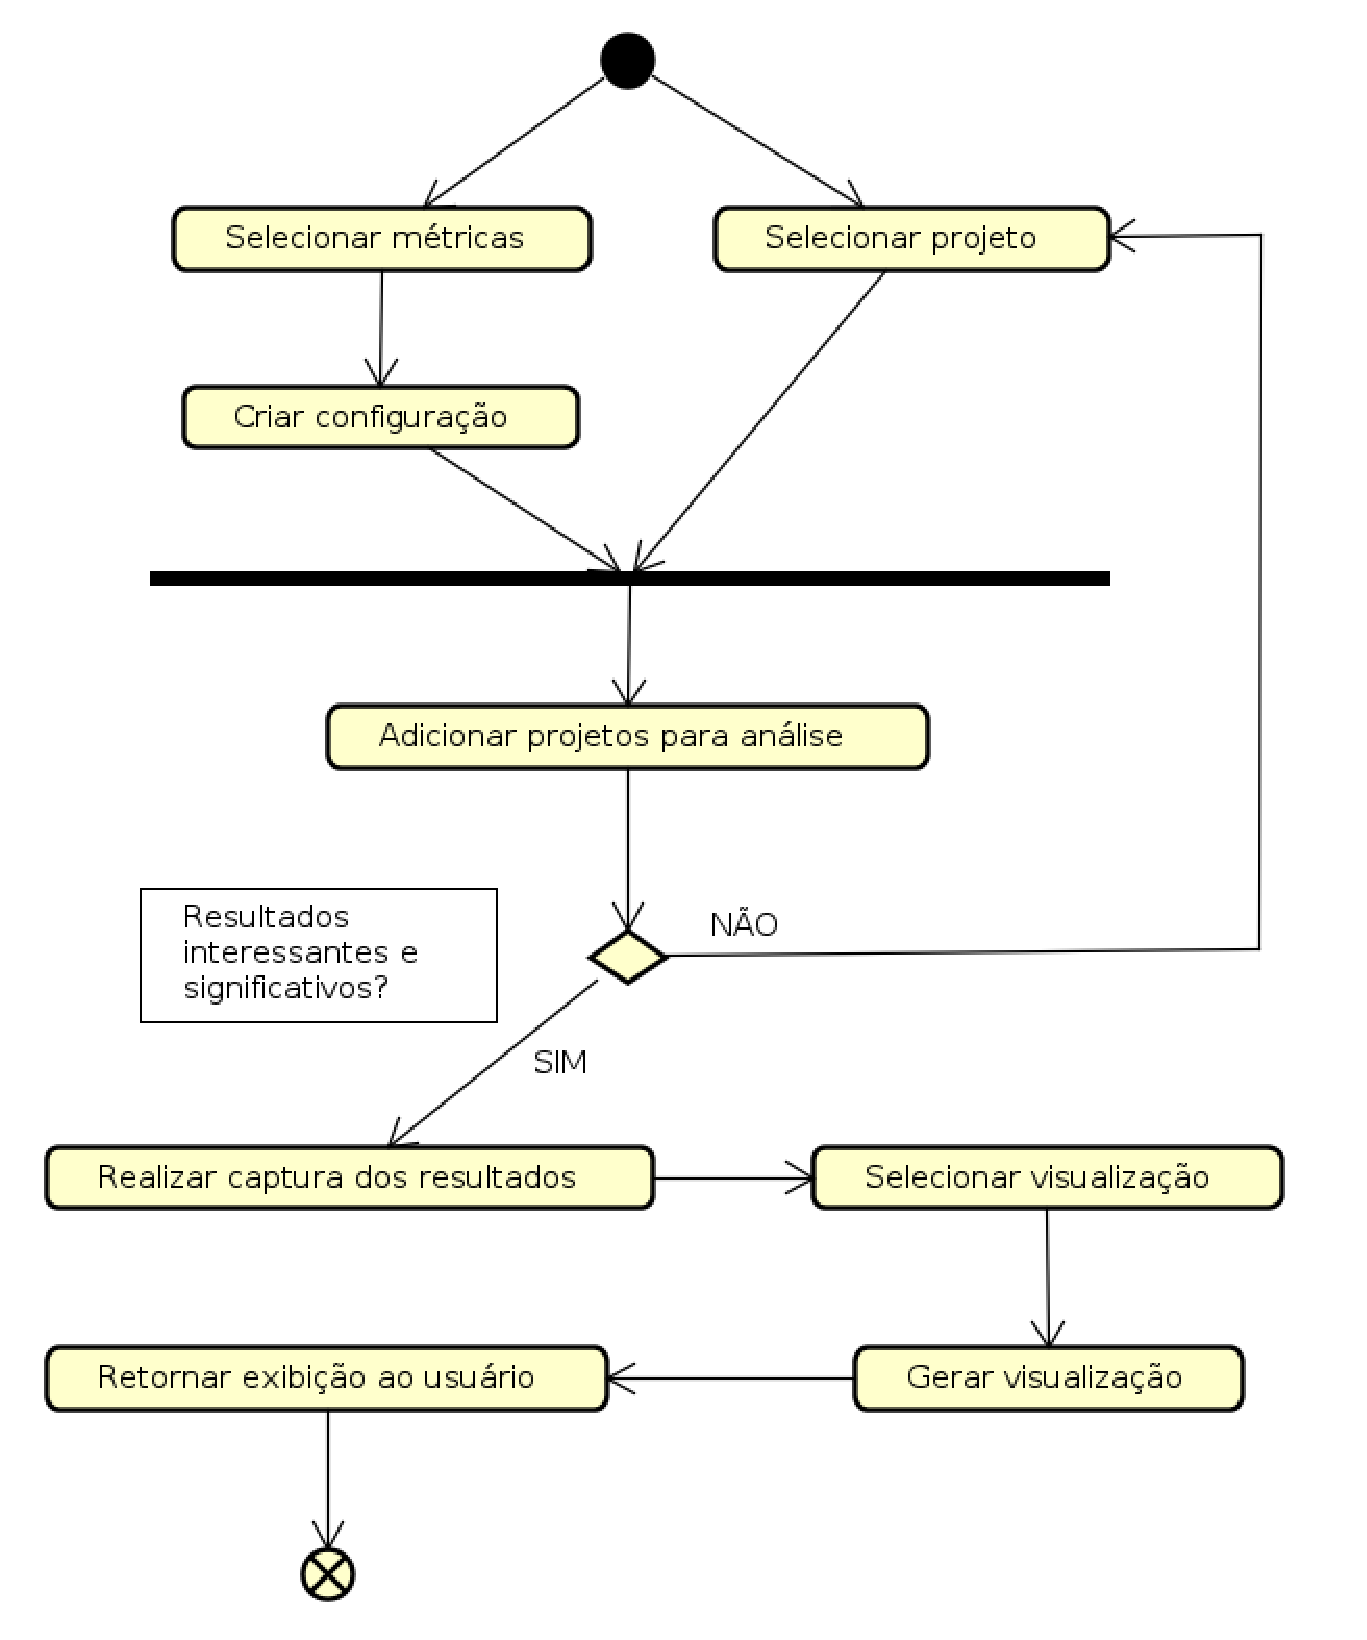
\includegraphics[keepaspectratio=true,scale=0.5]
    {figuras/metodotologia_atividades.eps}
  \caption{Encadeamento das etapas da atividade de contribuição tecnológica}
  \label{fig:metodotologia_atividades}
\end{figure}

\begin{enumerate}
  \item \textbf{Selecionar métricas}: Selecionar as métricas com maior nível de
  similaridade e afinidade com os objetivos de qualidade conhecidos.

  \item \textbf{Criar configuração}: Criar o contêiner em as métricas
  selecionadas estarão presentes. A configuração servirá para a associação aos
  projetos selecionados e a abstração de alto nível da visualização desejada.
  Criação esta seja em ambiente de desenvolvimento, seja no próprio Mezuro em
  produção.

  \item \textbf{Selecionar projetos}: Selecionar quais projetos que se melhor se
  adequem às métricas selecionadas e/ou possivelmente forneçam dados
  interessantes e significativos para a geração da visualização. Por exemplo:
  se as métricas selecionadas forem específicos de terminada linguagem, os
  projetos devem necessariamente terem seus códigos com maioria da escrita
  nessa linguagem. O número ideal é de três projetos, podendo conter a
  combinação entre, projetos que são reconhecidos por possuírem uma boa
  organização, com outros que são reconhecidos por não conterem determinado
  nível de qualidade.

  \item \textbf{Adicionar projetos para análise}: Adicionar projetos como um
  novo repositório para análise na plataforma Mezuro.

  \item \textbf{Realizar captura dos resultados}: Uma vez que os resultados
  forem interessantes e significativos, será feita a captura (parser) desses
  dados utilizando talvez as Ruby Gems Sinatra ou Seed\_dump.

  \item \textbf{Selecionar visualização}: Antes de gerar a visualização, será
  feito a escolha da melhor visualização dado o contexto, relevância e
  granularidade dos dados resultantes da análise. Levando em consideração também
  as técnicas estudadas e um número finito pré-estabelecidos de visualizações.

  \item \textbf{Gerar visualização}: utilizar biblioteca de criação de
  visualização para criação da representação alternativa dos dados da análise.

  \item \textbf{Retornar exibição ao usuário}: Nesta fase será elaborada o
  retorno da visualização ao usuário, como mencionado antes, seja em uma nova
  página ou nas informações gerais do repositório analisado.
\end{enumerate}

\section{Seleção das Métricas}

% TODO: selecionar métricas com certo nível de similaridade.
% TODO: citar aqui talvez Michelle Lanza e R Marinescu - software metrics

% capitulo 3 - metodologias, vem o mezuro
\chapter{Resultados Preliminares}

\section{Mezuro: Prezento}

Como dito no capítulo anterior, o Prezento é a camada da interface web do
Mezuro. Desenvolvido em Ruby on Rails, atualmente utiliza as versões 2.3.0 do
Ruby e 4.2.4 do Rails. Versões estas que estão em constante mudança, pois os
autores têm como intuito usufruir o que há de mais recente das funcionalidades
dessa tecnologia. Esta será a principal camada trabalhada neste trabalho de
conclusão de curso, pois é
nela que há a interação com o usuário. Possivelmente será utilizado um botão que
possibilitará ao usuário ter acesso e interagir com a visualização gráfica do
resultado da análise estática na mesma página ou em outra. As Figuras
\ref{fig:exmplo_disposicao_botao_visualizacao_1} e
\ref{fig:exmplo_disposicao_botao_visualizacao_2} mostram possíveis localizações
para este botão.

% TODO: atualizar estas imagens e DESTACAR botôes

\begin{figure}[!htb]
	\centering
    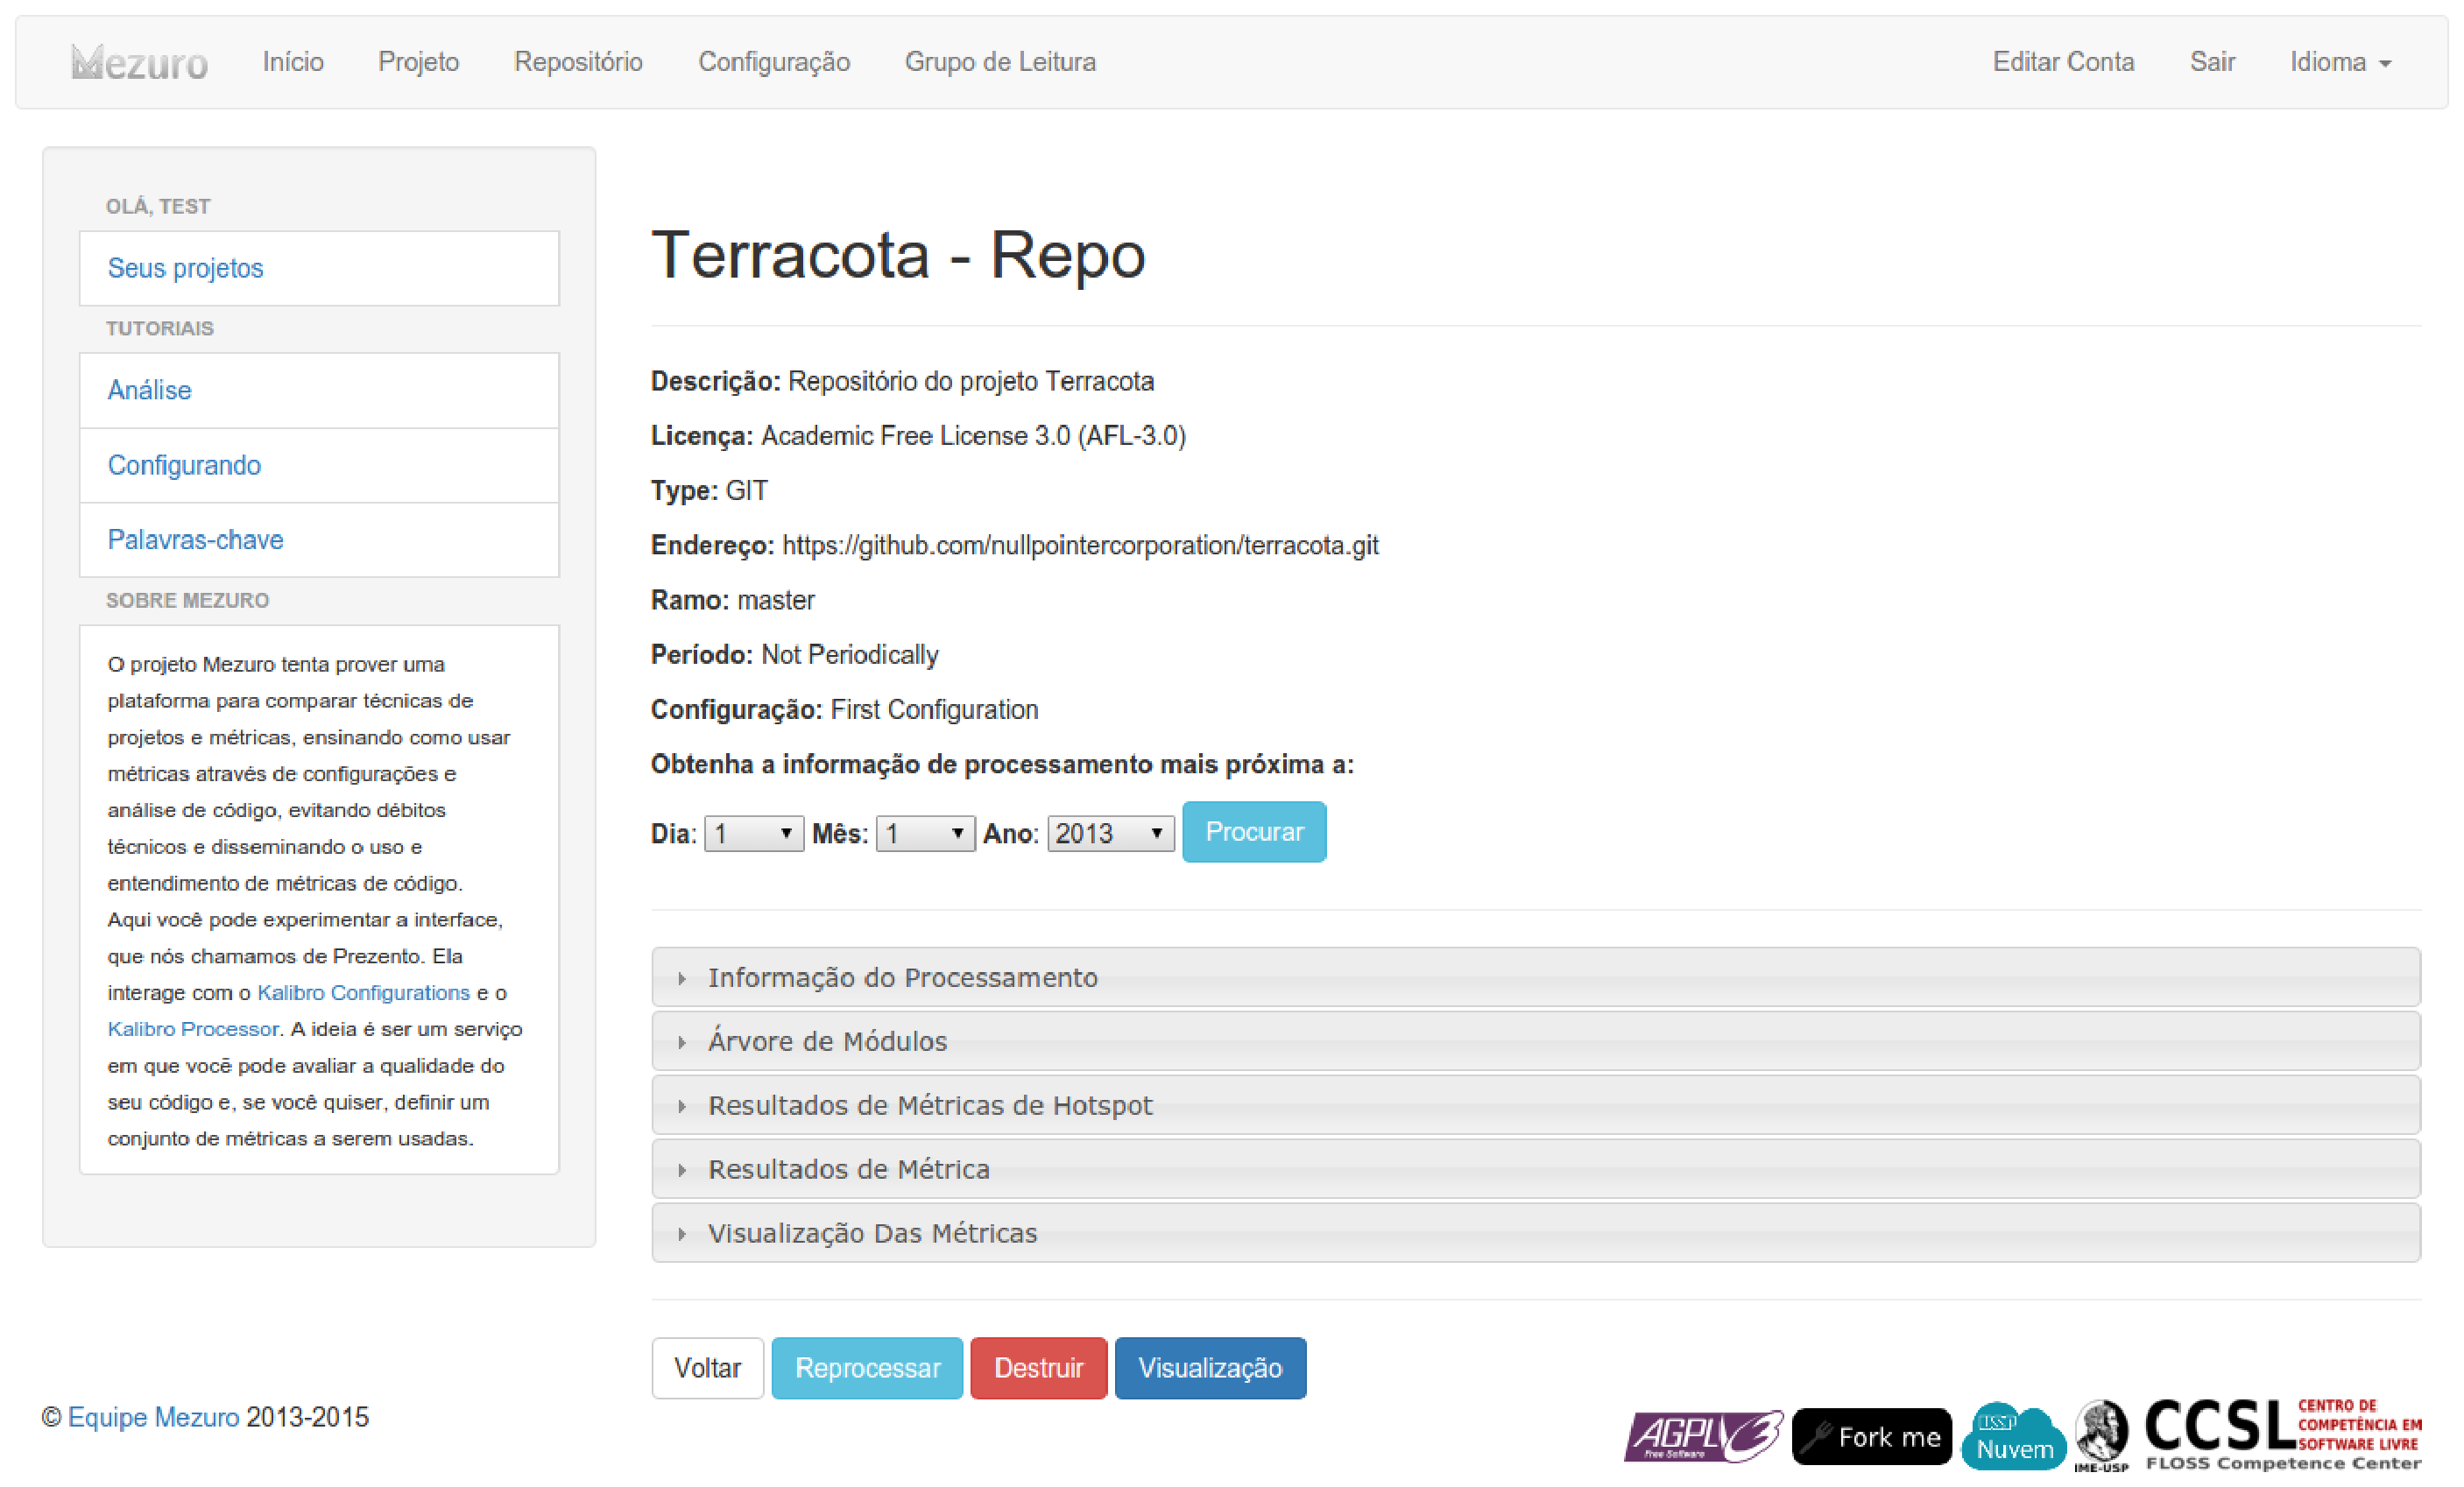
\includegraphics[keepaspectratio=true,scale=0.33]
    {figuras/exmplo_disposicao_botao_visualizacao_1.eps}
  \caption{Possíveis disposições dos botões de acesso à visualização (recolhido)}
  \label{fig:exmplo_disposicao_botao_visualizacao_1}
\end{figure}

\begin{figure}[!htb]
	\centering
    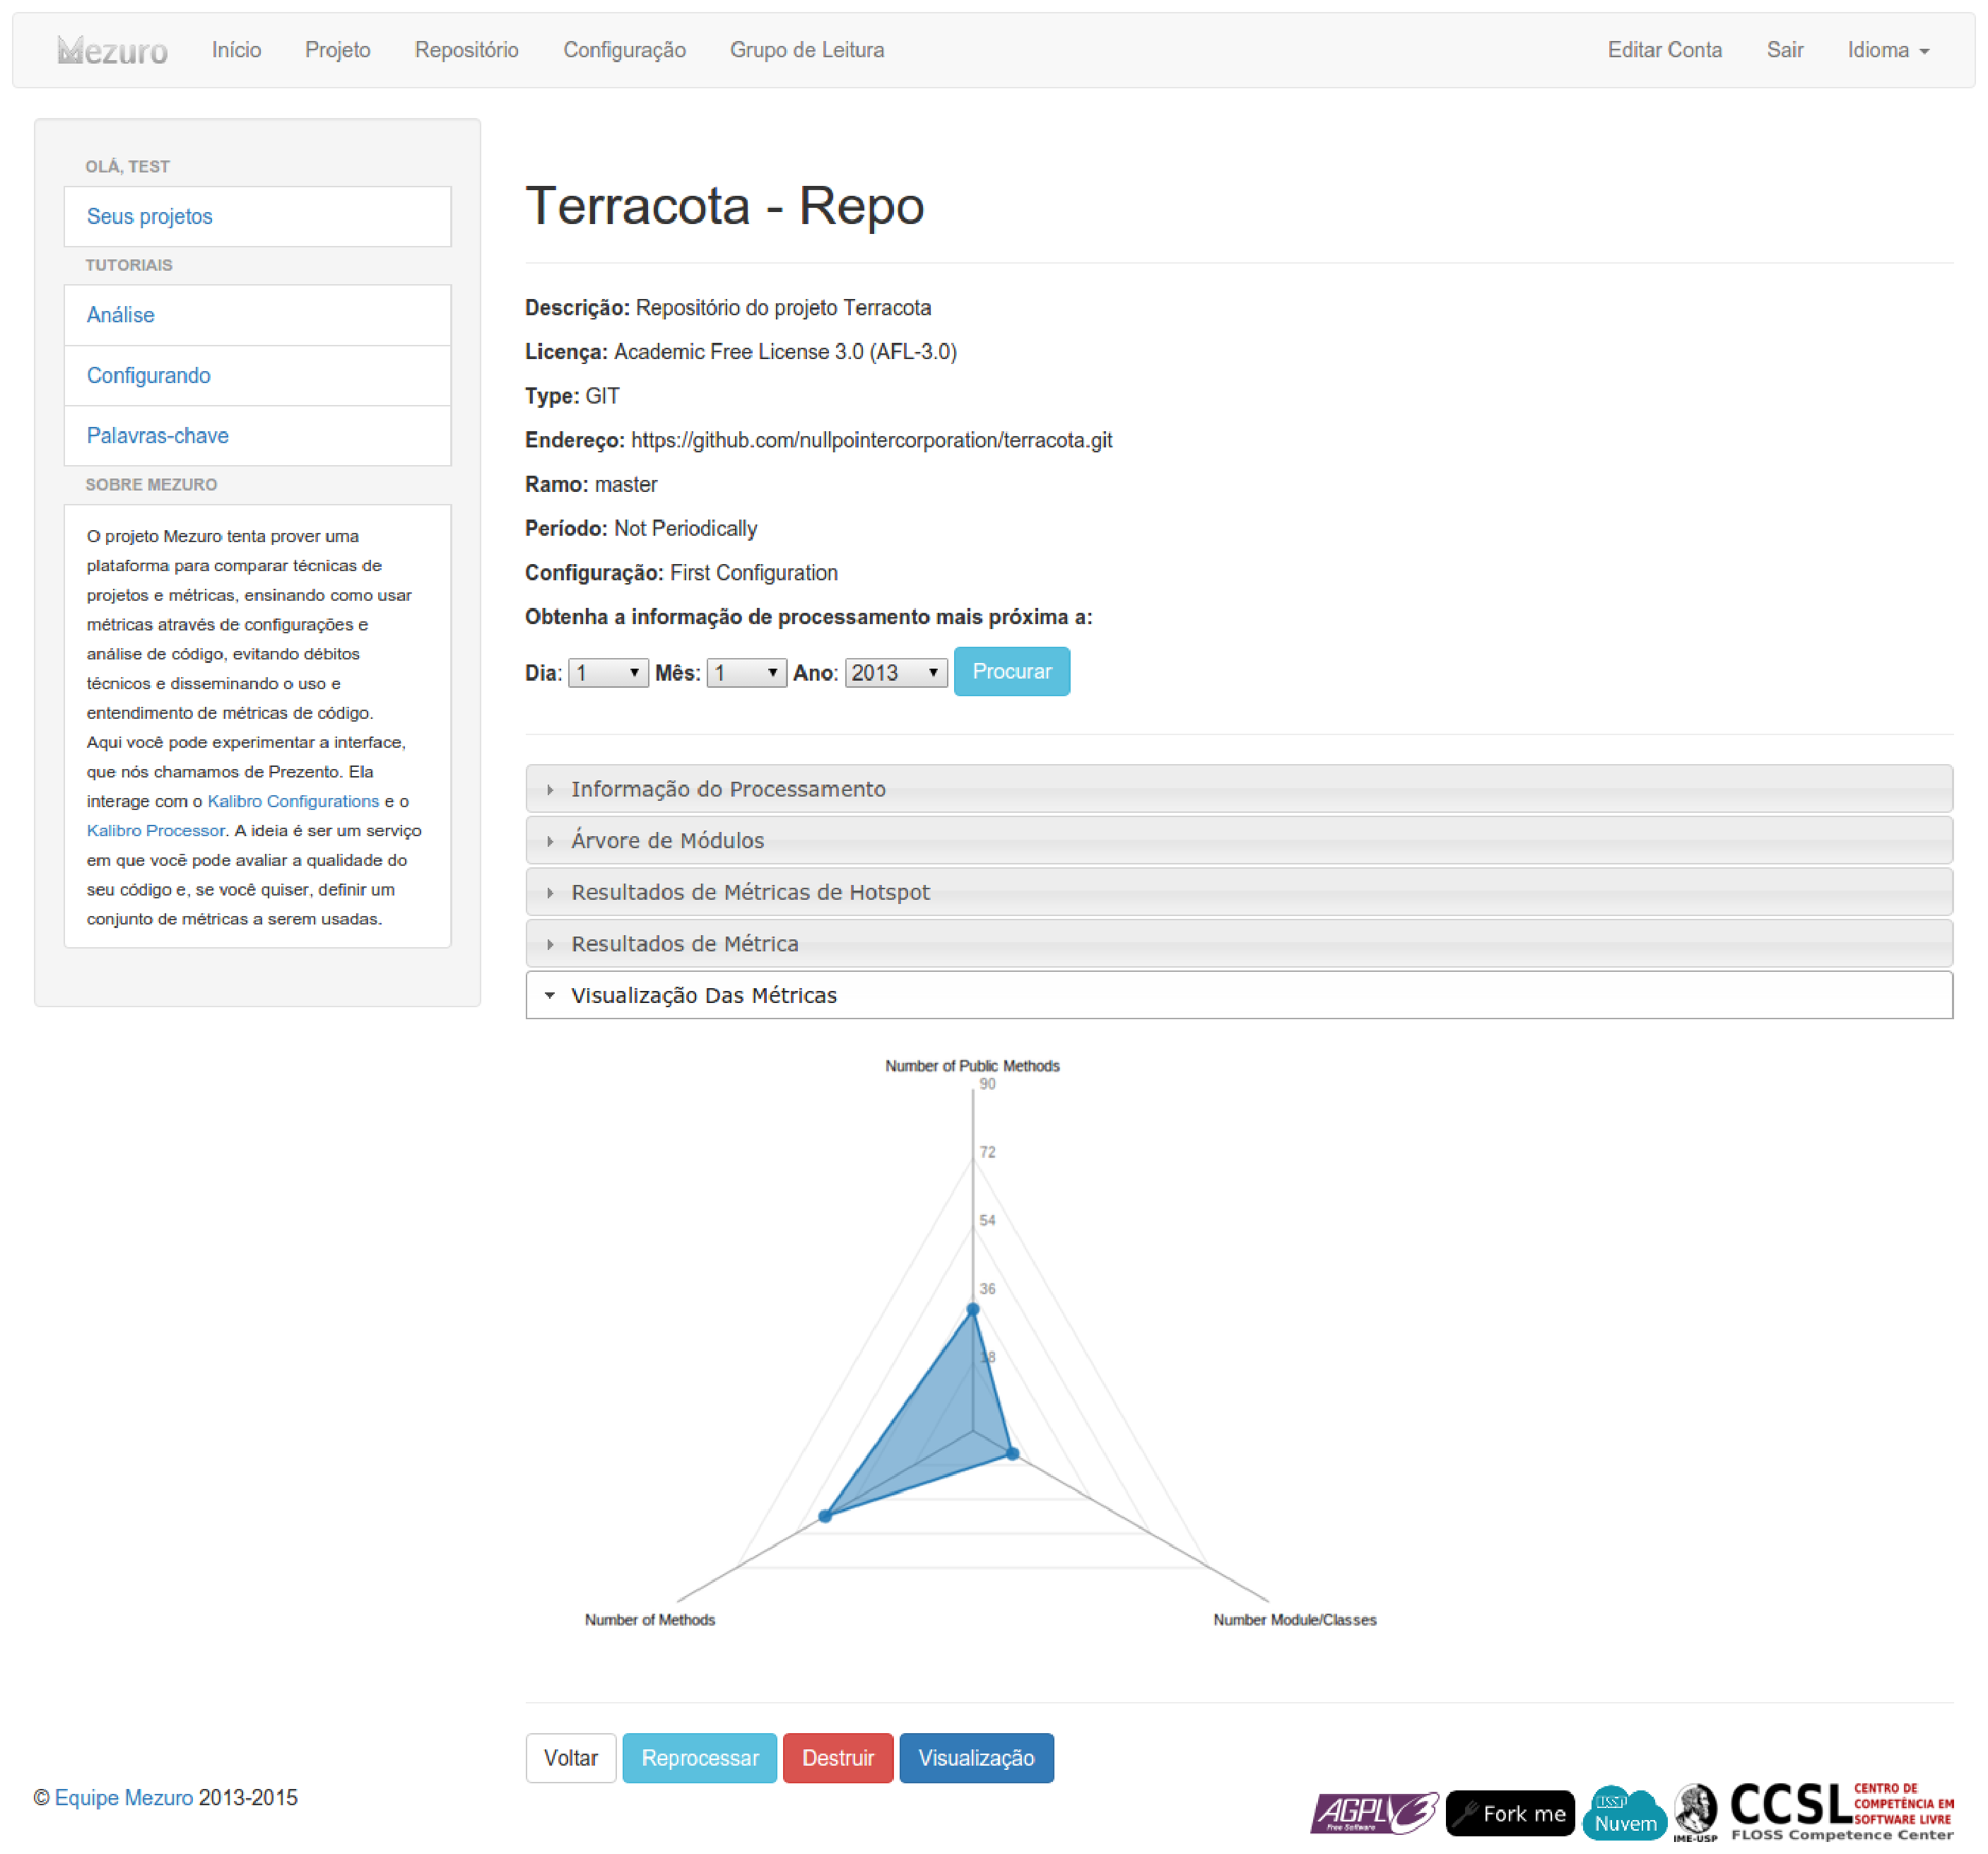
\includegraphics[keepaspectratio=true,scale=0.33]
    {figuras/exmplo_disposicao_botao_visualizacao_2.eps}
  \caption{Possíveis disposições dos botões de acesso à visualização
  (expandido) (adptado) \cite{filgueiras2014mezuro}}
  \label{fig:exmplo_disposicao_botao_visualizacao_2}
\end{figure}

\newpage

As Figuras \ref{fig:controllers_complete} e \ref{fig:models_complete} mostram os
diagramas das camadas de Controle e de Modelo do Prezento. Foram geradas com a
\textit{gem} RailRoady\footnote{\url{http://railroady.prestonlee.com/}}.

% TODO: atualizar estes diagramas

\begin{figure}[!htb]
	\centering
    \includegraphics[keepaspectratio=true,scale=0.33]
    {figuras/controllers_complete.eps}
  \caption{Diagrama da Camada de Controle}
  \label{fig:controllers_complete}
\end{figure}

\begin{figure}[!htb]
	\centering
    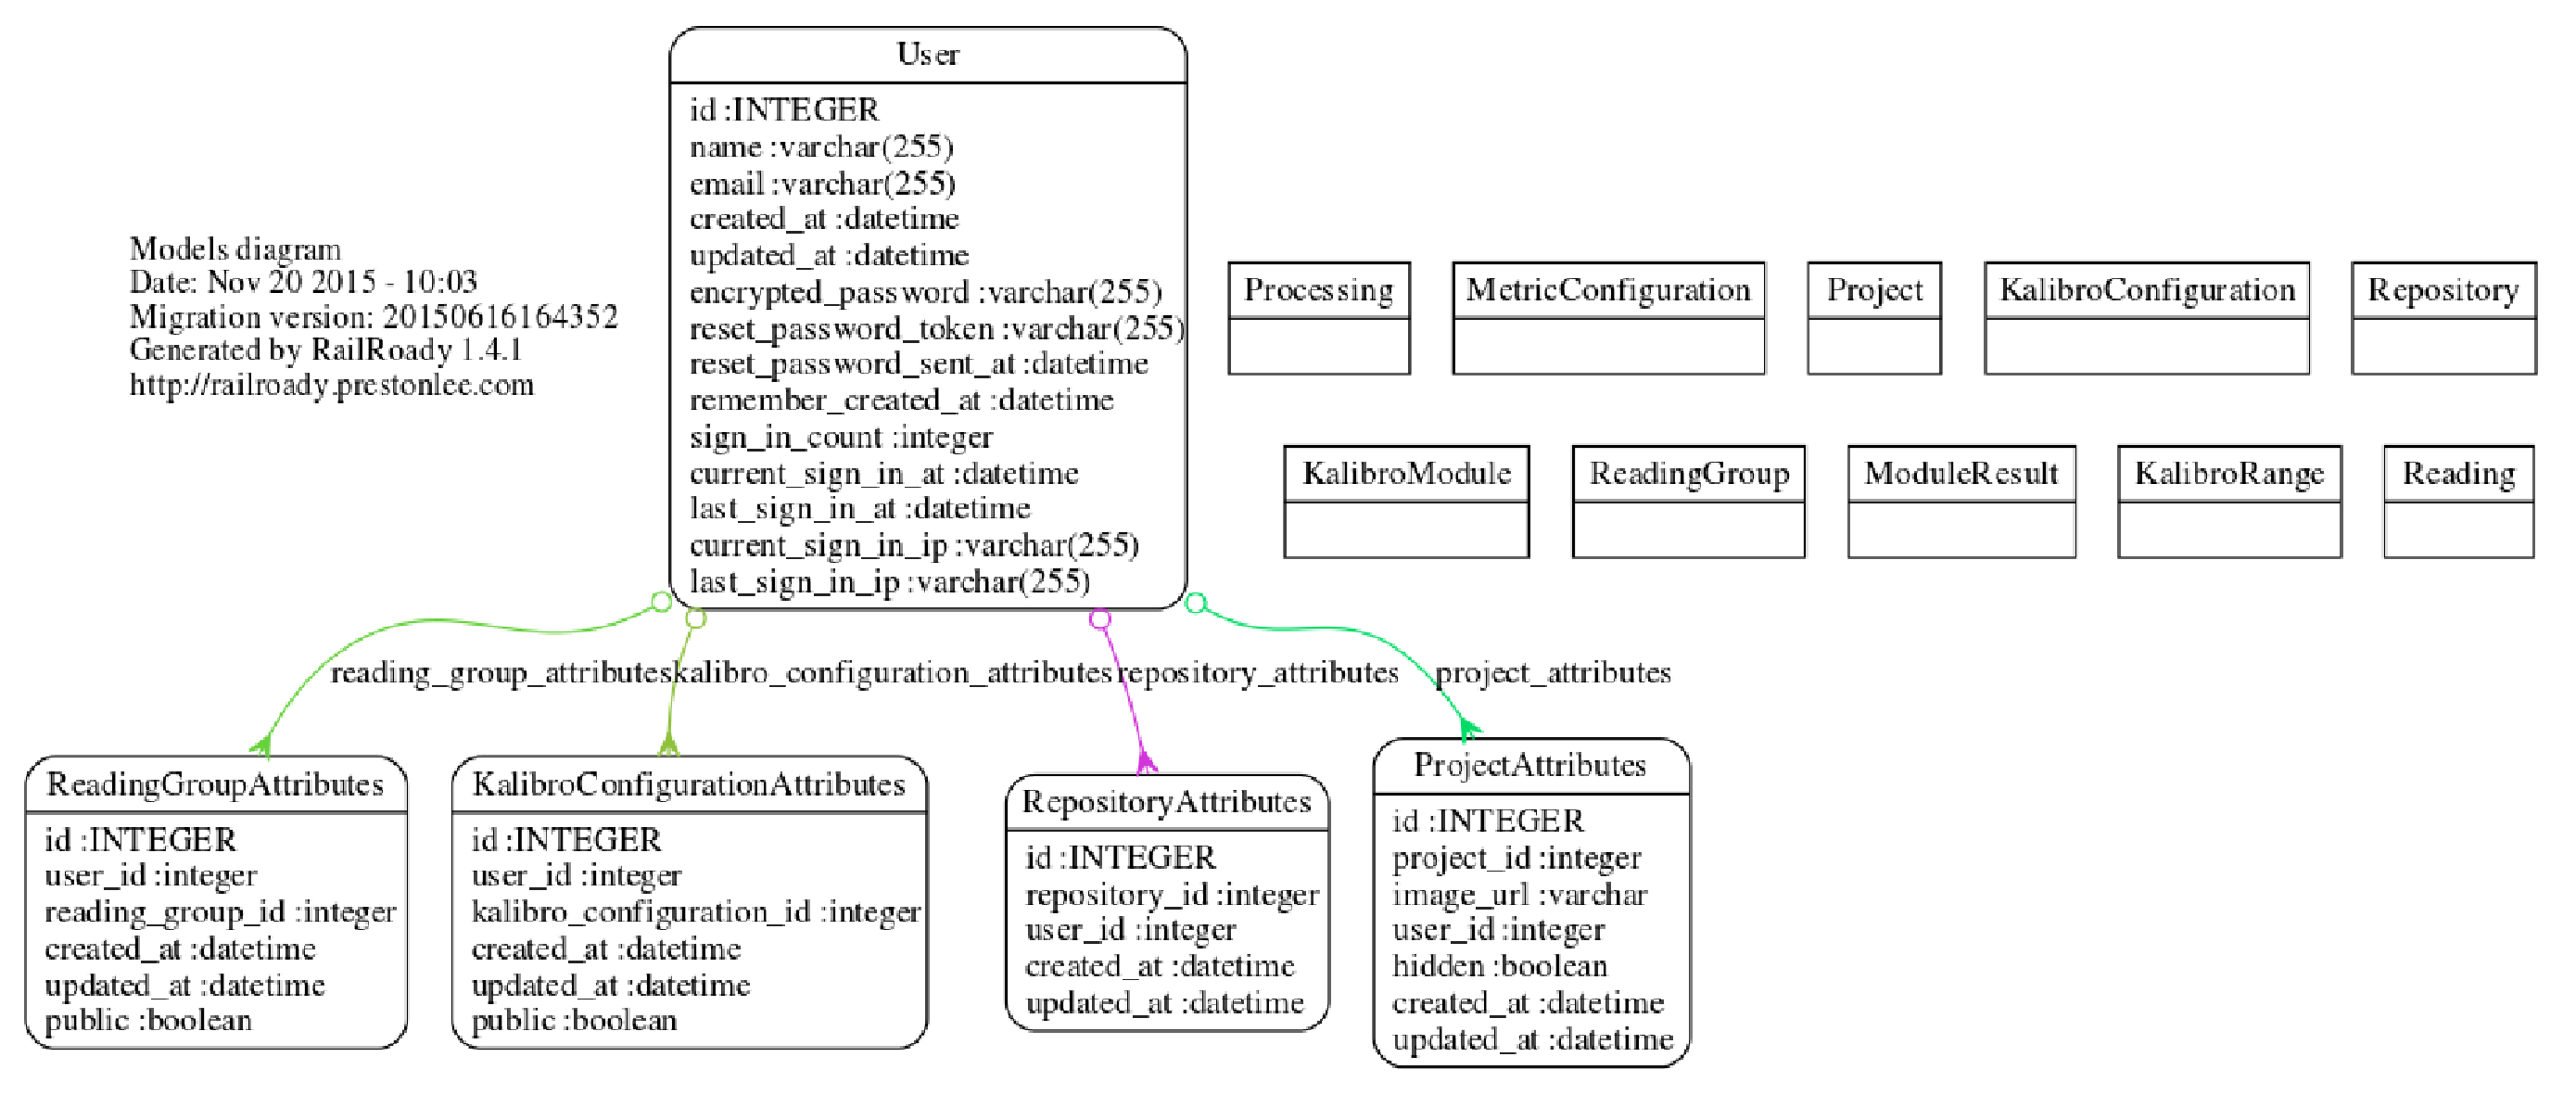
\includegraphics[keepaspectratio=true,scale=0.35]
    {figuras/models_complete_v2.eps}
  \caption{Diagrama da Camada de Modelo}
  \label{fig:models_complete}
\end{figure}

\newpage

\section{D3 - Data-Driven Documents}

D3.js (\textit{Data-Driven-Documents}) é uma biblioteca Javascript construída
inicialmente por \citeonline{bostock2011d3}, que tem como um dos seus objetivos
principais a produção de visualizações dinâmicas e interativas para a Web. Ela
faz uso de várias tecnologias vastamente utilizadas: HTML (para o conteúdo das
páginas), SVG (para descrição de gráficos vetoriais) e CSS (para estética das
páginas). A Figura \ref{fig:d3_gears} é um exemplo de como esse uso (ou
interação) é feito. Esta biblioteca permite ao programador manipular o Modelo de
Objeto de Documento (do inglês, \textit{Document Object Model} - DOM), para
modificar determinada seleção de elementos na página. Essa modificação, seja
adição ou remoção de elementos, depende dos dados de entrada e é onde a
aplicação de transformações dinâmicas é feita. Os autores idealizaram a união de
três preocupações: compatibilidade, depuração e desempenho \cite{bostock2011d3}.

\begin{figure}[!htb]
	\centering
    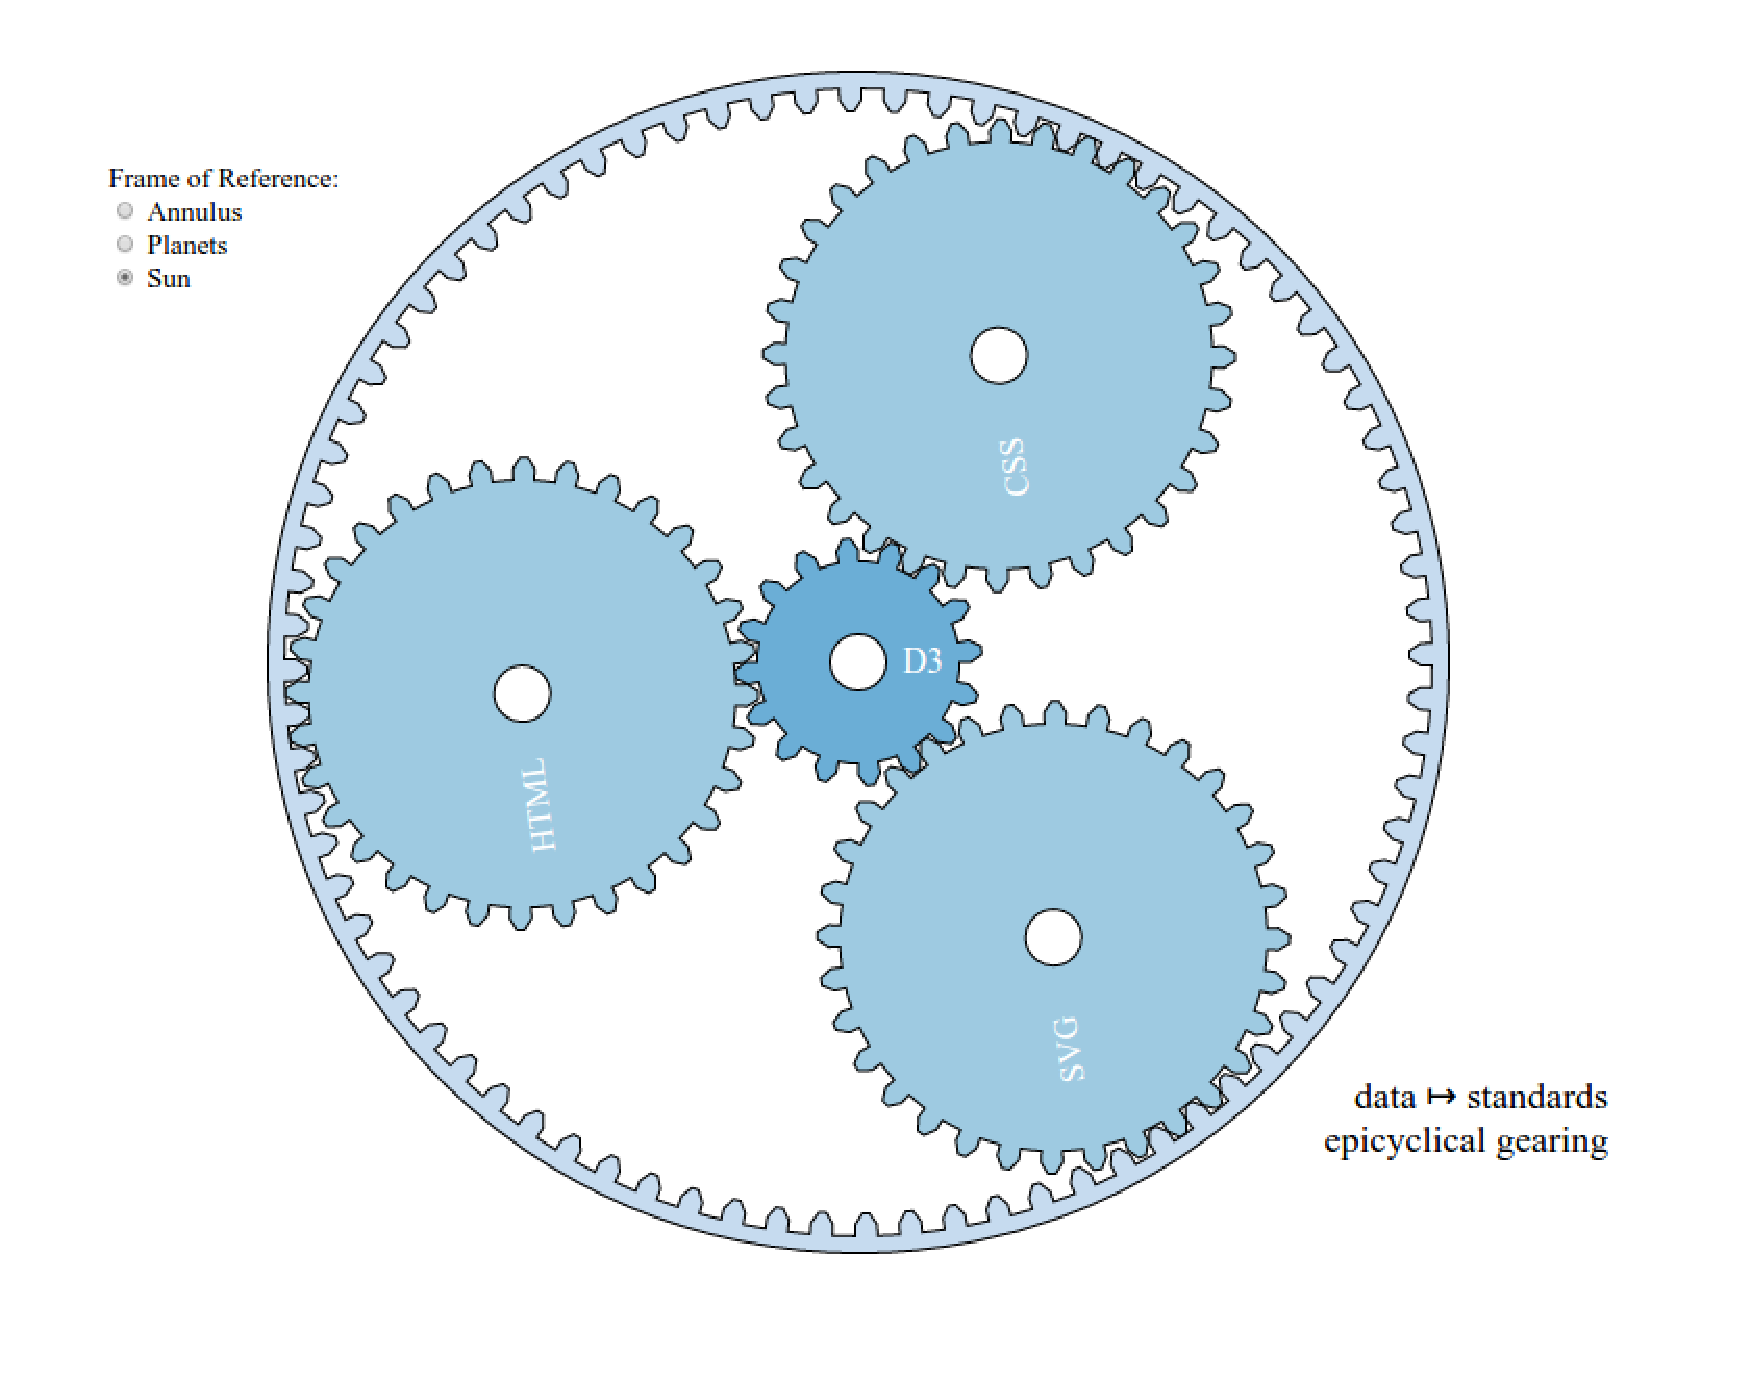
\includegraphics[keepaspectratio=true,scale=0.5]
    {figuras/d3_gears.eps}
  \caption{Exemplificação do Uso das Tecnologias pela D3.js \cite{michaeld3}}
  \label{fig:d3_gears}
\end{figure}

A biblioteca D3.js é licenciada sob a \textit{BSD licenses}, que é compatível
com a licença do Mezuro (\textit{AGPL} - \textit{Version} 3) e possui uma vasta
galeria de exemplos que podem se adaptar ao proposto neste trabalho.

\begin{figure}[!htb]
	\centering
    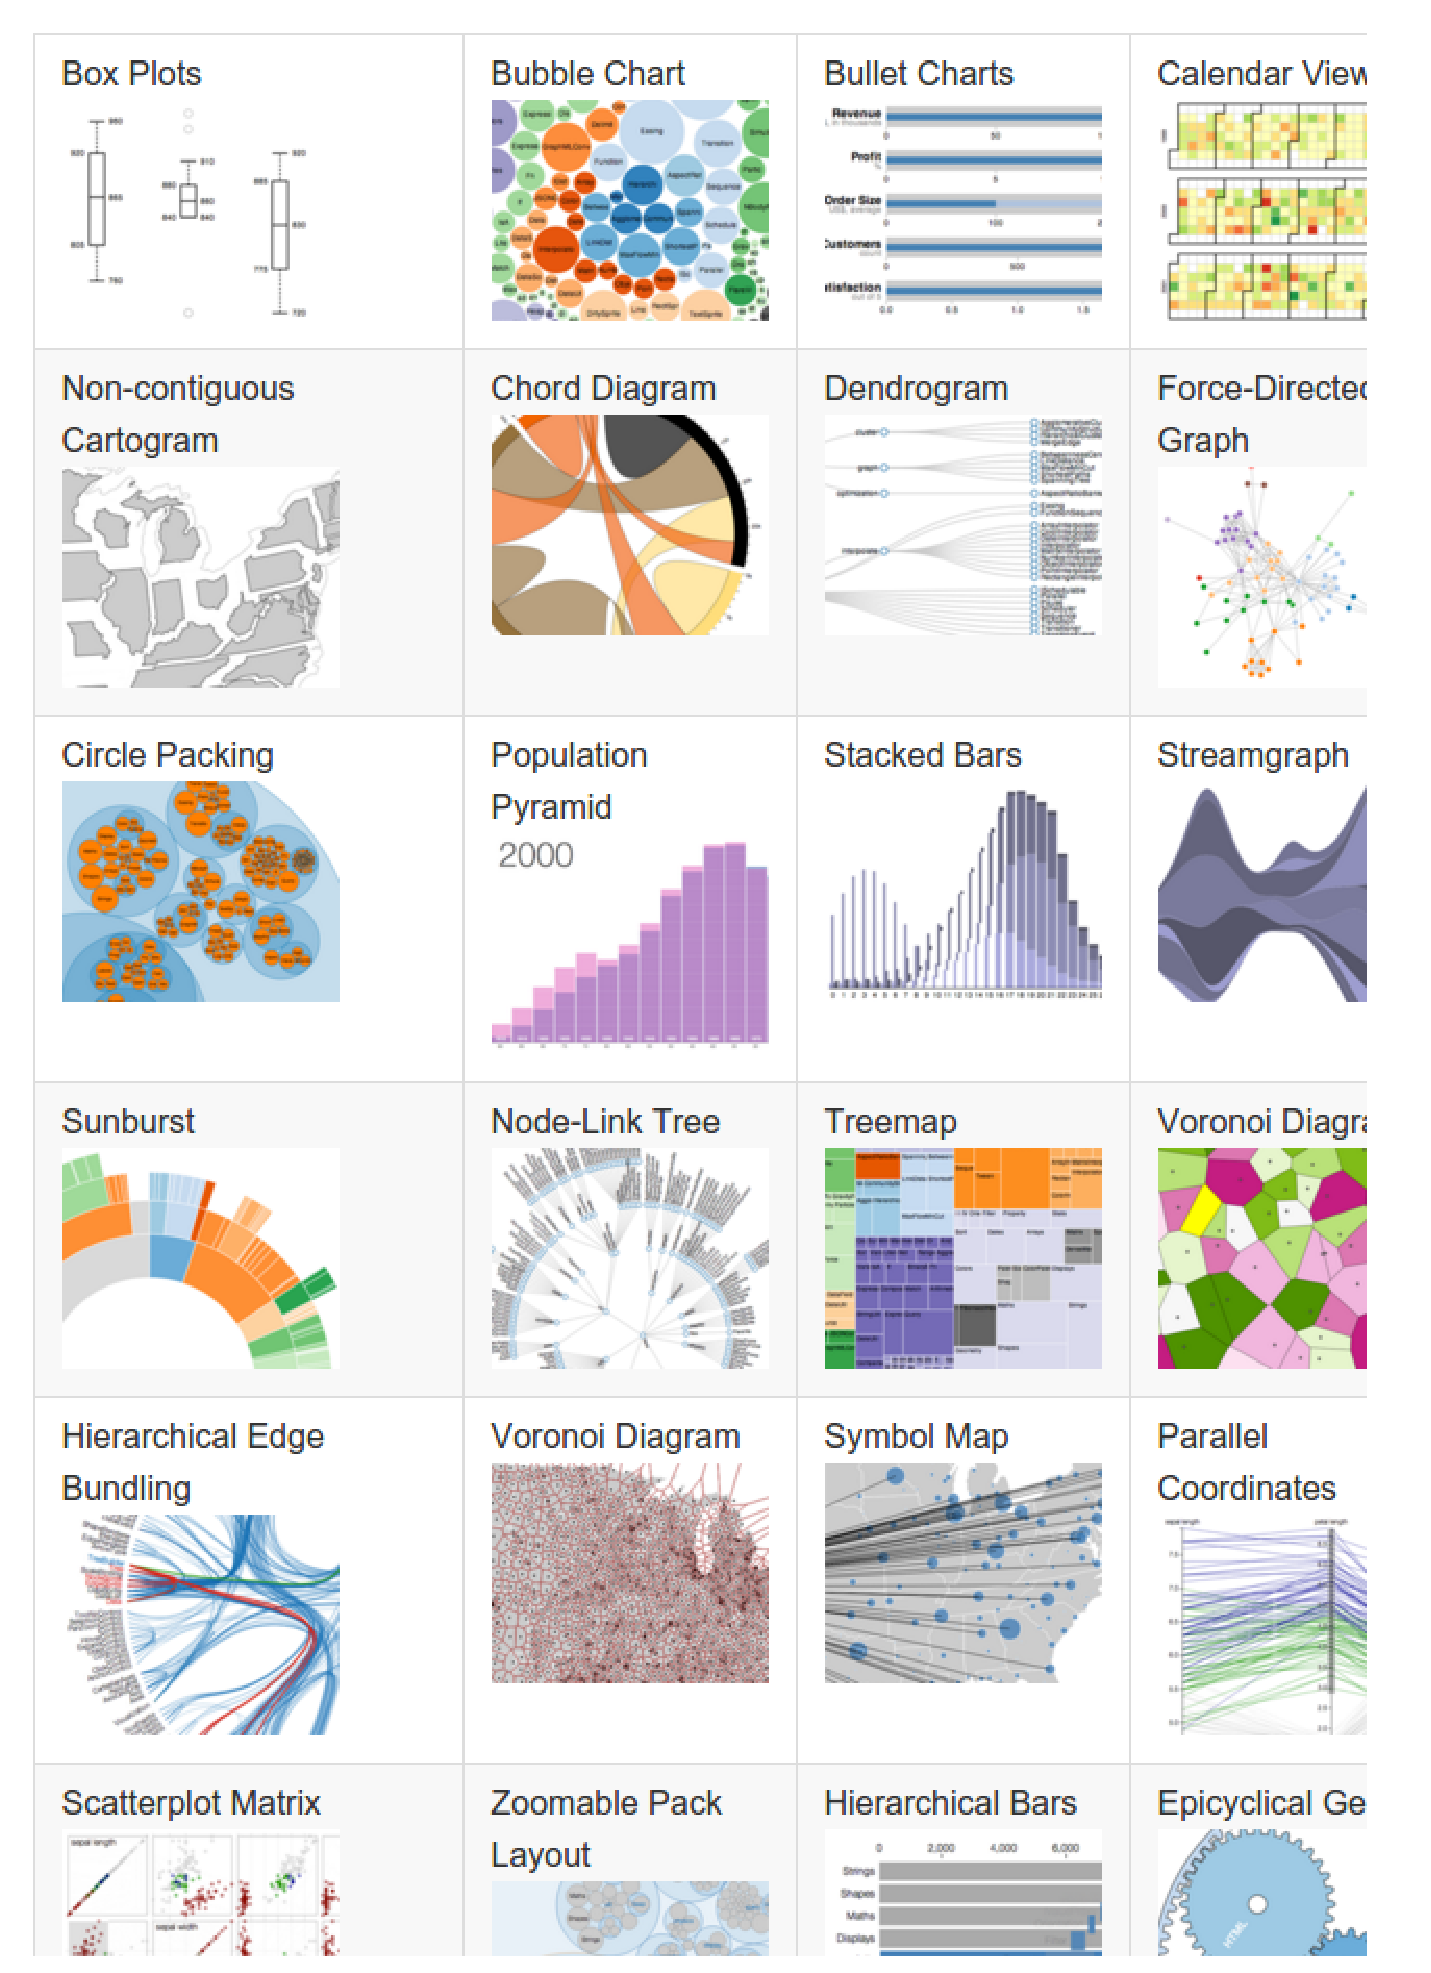
\includegraphics[keepaspectratio=true,scale=0.5]
    {figuras/d3_gallery.eps}
  \caption{Galeria de Exemplos da biblioteca D3.js \cite{galleryD3}}
  \label{fig:d3_gallery}
\end{figure}

https://github.com/mbostock/d3/wiki/Gallery

\section{Exemplo de Uso}

% TODO: escolher 3 projetos para serem alvo
% TODO: escolher quais métricas

\subsection{Resultados Econtrados}

\section{Visualização - Gráfico Radar}

\chapter[Conclusão]{Conclusão}

\section{Seção 1}

\section{Seção 2}

\bookmarksetup{startatroot}

\postextual

\bibliography{bibliografia}
\begin{apendicesenv}

\partapendices

\chapter{Primeiro Apêndice}
\label{chap:apendiceA}

Resultado completo da pesquisa realizada.

\begin{figure}[!htb]
	\centering
    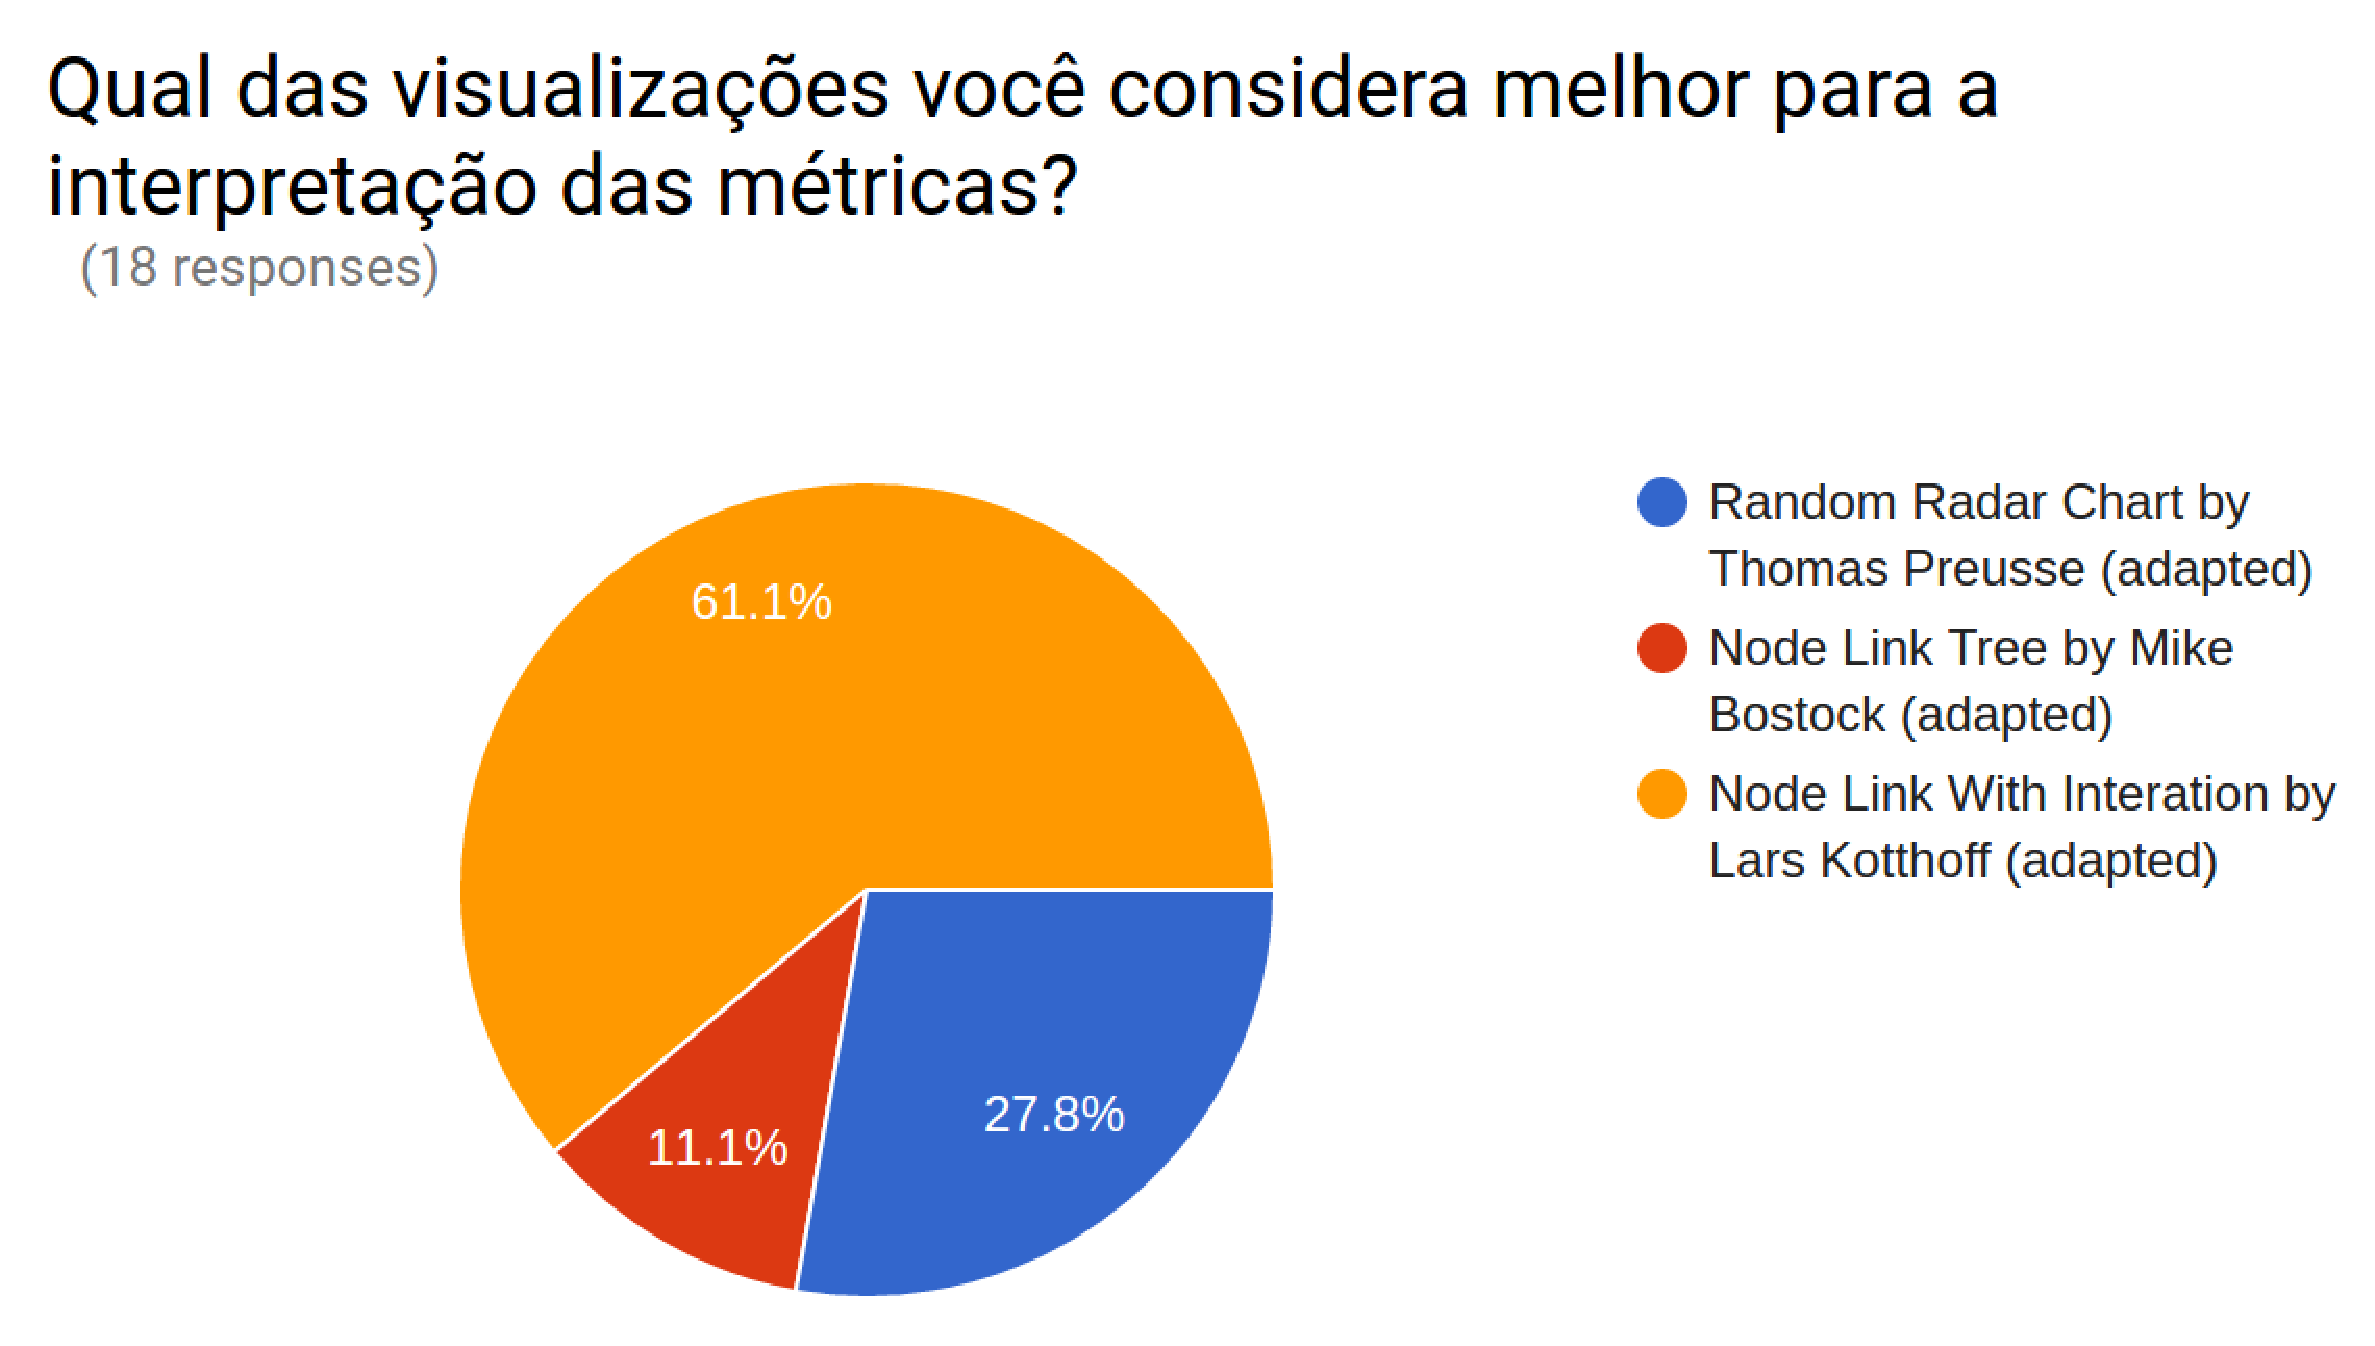
\includegraphics[keepaspectratio=true,scale=0.35]
    {figuras/res1.eps}
  \caption{Visualização considerada de melhor interpretação}
  \label{fig:res1}
\end{figure}

\begin{figure}[!htb]
	\centering
    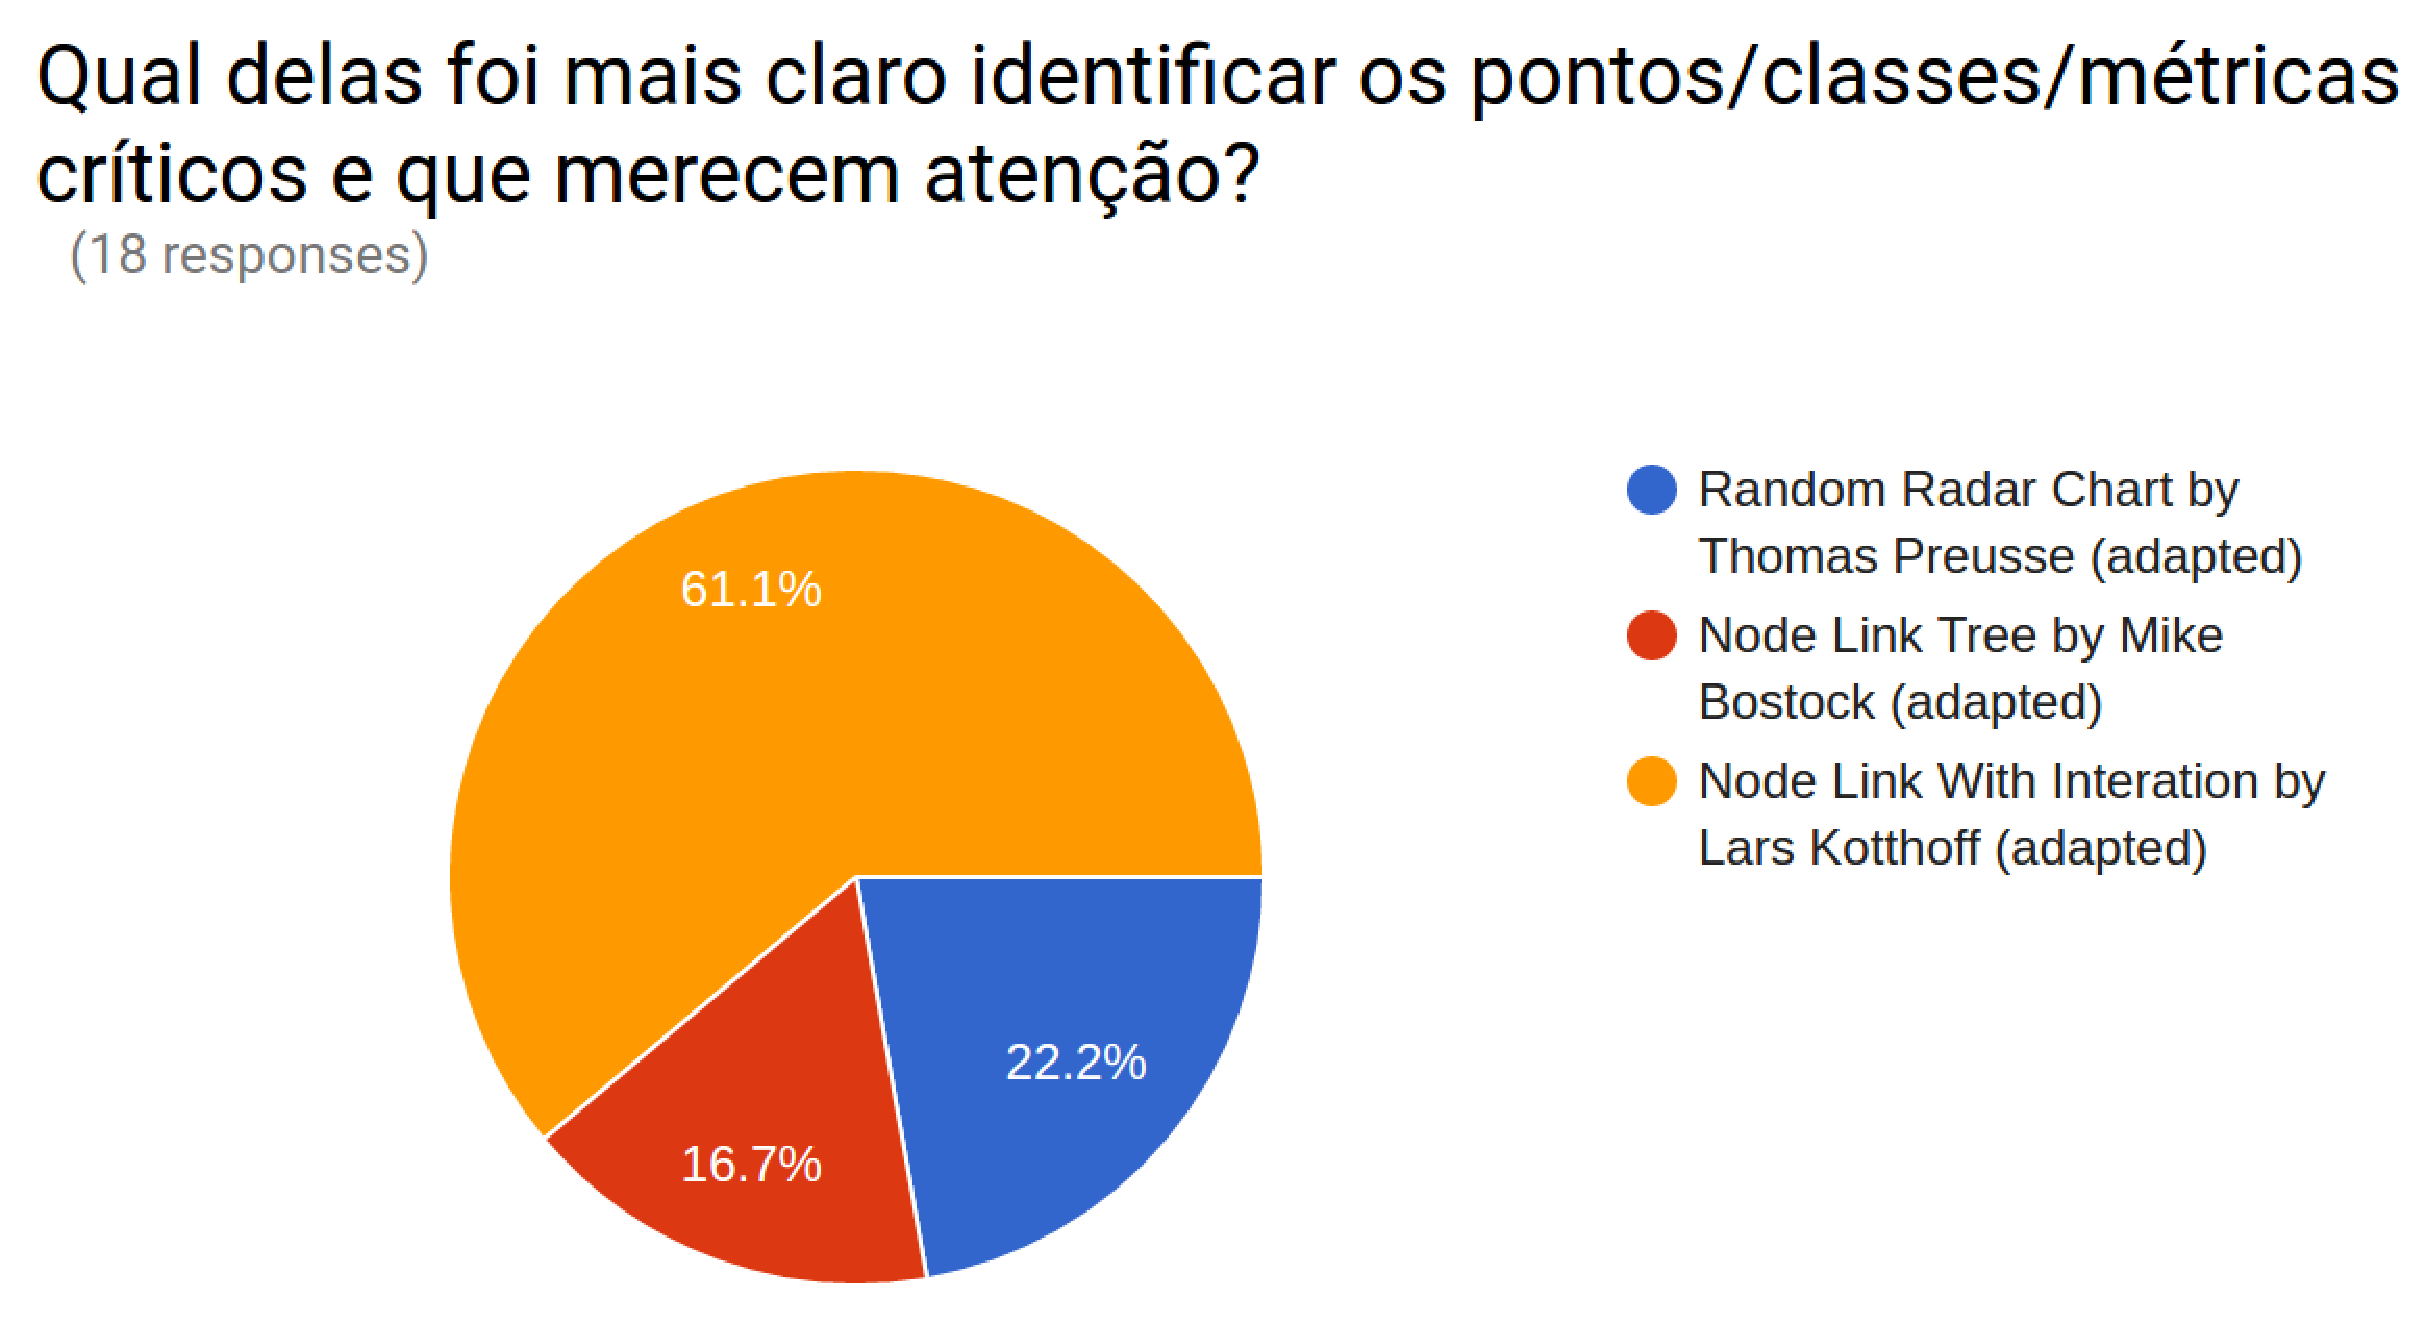
\includegraphics[keepaspectratio=true,scale=0.35]
    {figuras/res2.eps}
  \caption{Visualização com maior clareza na identificação dos pontos críticos}
  \label{fig:res2}
\end{figure}

Comentários, críticas e sugestões (6 respostas). Todas as respostas foram
anônimas:

\textit{``Se o método de Node With Interations, do Lars Kotthoff, começasse com
alguns nós expandidos, ele seria o melhor (na minha opinião) de longe. Como
isso não está ocorrendo, ele ainda continua melhor (na minha opinião), mas os
outros dois são mais claros para se ver o resultado final a respeito das
métricas.''}

\textit{``O primeiro eu não entendi como funciona, se entendesse deve ser legal. O
segundo me deu dor de cabeça só de abrir a imagem e é ruim ficar virando a
cabeça e espremendo os olhos pra enxergar (tenho miopia)  O terceiro é legal
porque mostra tudo separadinho mas é um saco ter que clicar mil vezes pra ver
tudo.''}

\textit{``Poderia colocar uma opção de visualização: Node Link With Interation
by Lars Kotthoff de vizsualizar tudo de uma vez, um expand all.}

\textit{``Para a forma de visualização do Node Link With Interation by Lars
Kotthoff (adapted) seria interessante ter um aspecto de botão para a pessoa
saber que o elemento é para ser clicado.''}

\textit{``A nível de entendimento e clareza a visualização em Node Link With
Interation é a melhor, no entanto a que se apresenta de forma mais bonita é a
Node Link Tree, embora não seja tão intuitiva quanto a anterior. Além disso, a
No Link With Interation parece ter demonstrado ter capturado melhor as
necessidades, conforme a leitura das métricas, na medida em que visualmente
aponta mais valores em VERMELHO que a opção Node Link Tree. A Random Radar
Chart não evidencia valores. Não há uma escala, o que dificulta
o entendimento da gravidade da situação de uma determinada métrica.''}

\textit{``Node Link Tree by Mike Bostock é a melhor, mas para ser o mais claro é
preciso trabalhar melhor com as cores usando os valores agregados de métricas.
Coloque cores em todos os nós do grafo de acordo com o grade.''}

\end{apendicesenv}

\begin{anexosenv}

\partanexos

\chapter{Primeiro Anexo}
\label{chap:anexoA}

Resultados completos da pesquisa realizada.

\begin{figure}[!htb]
	\centering
    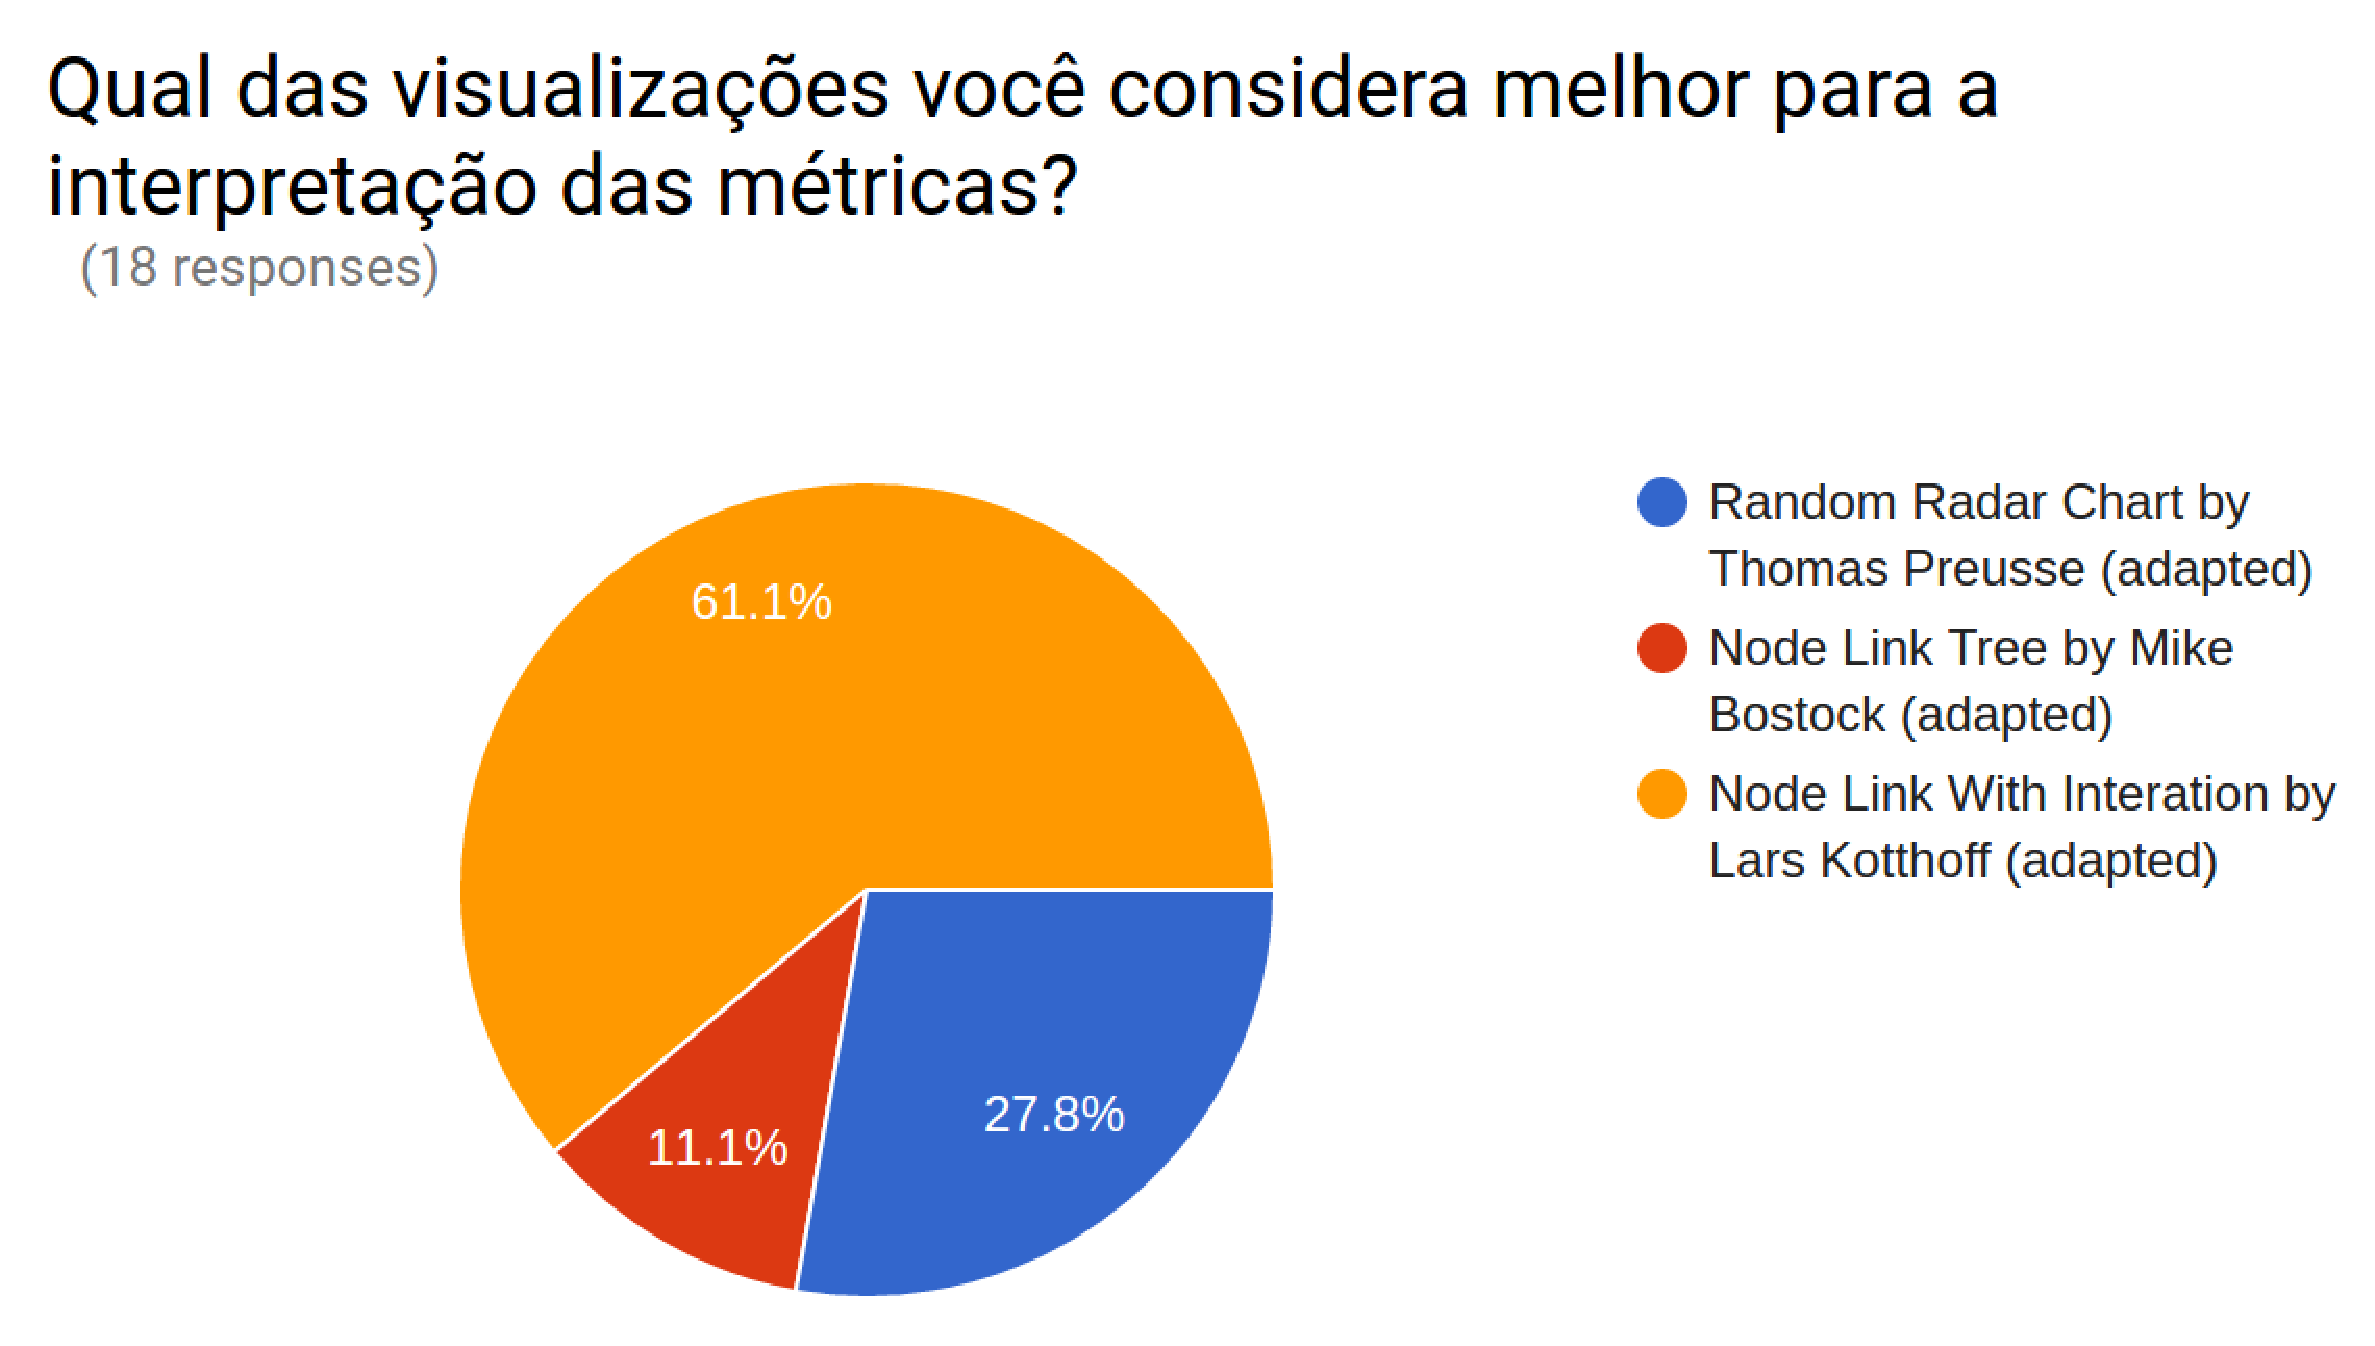
\includegraphics[keepaspectratio=true,scale=0.35]
    {figuras/res1.eps}
  \caption{Respostas para qual visualização foi considerada de melhor
  interpretação}
  \label{fig:res1}
\end{figure}

\begin{figure}[!htb]
	\centering
    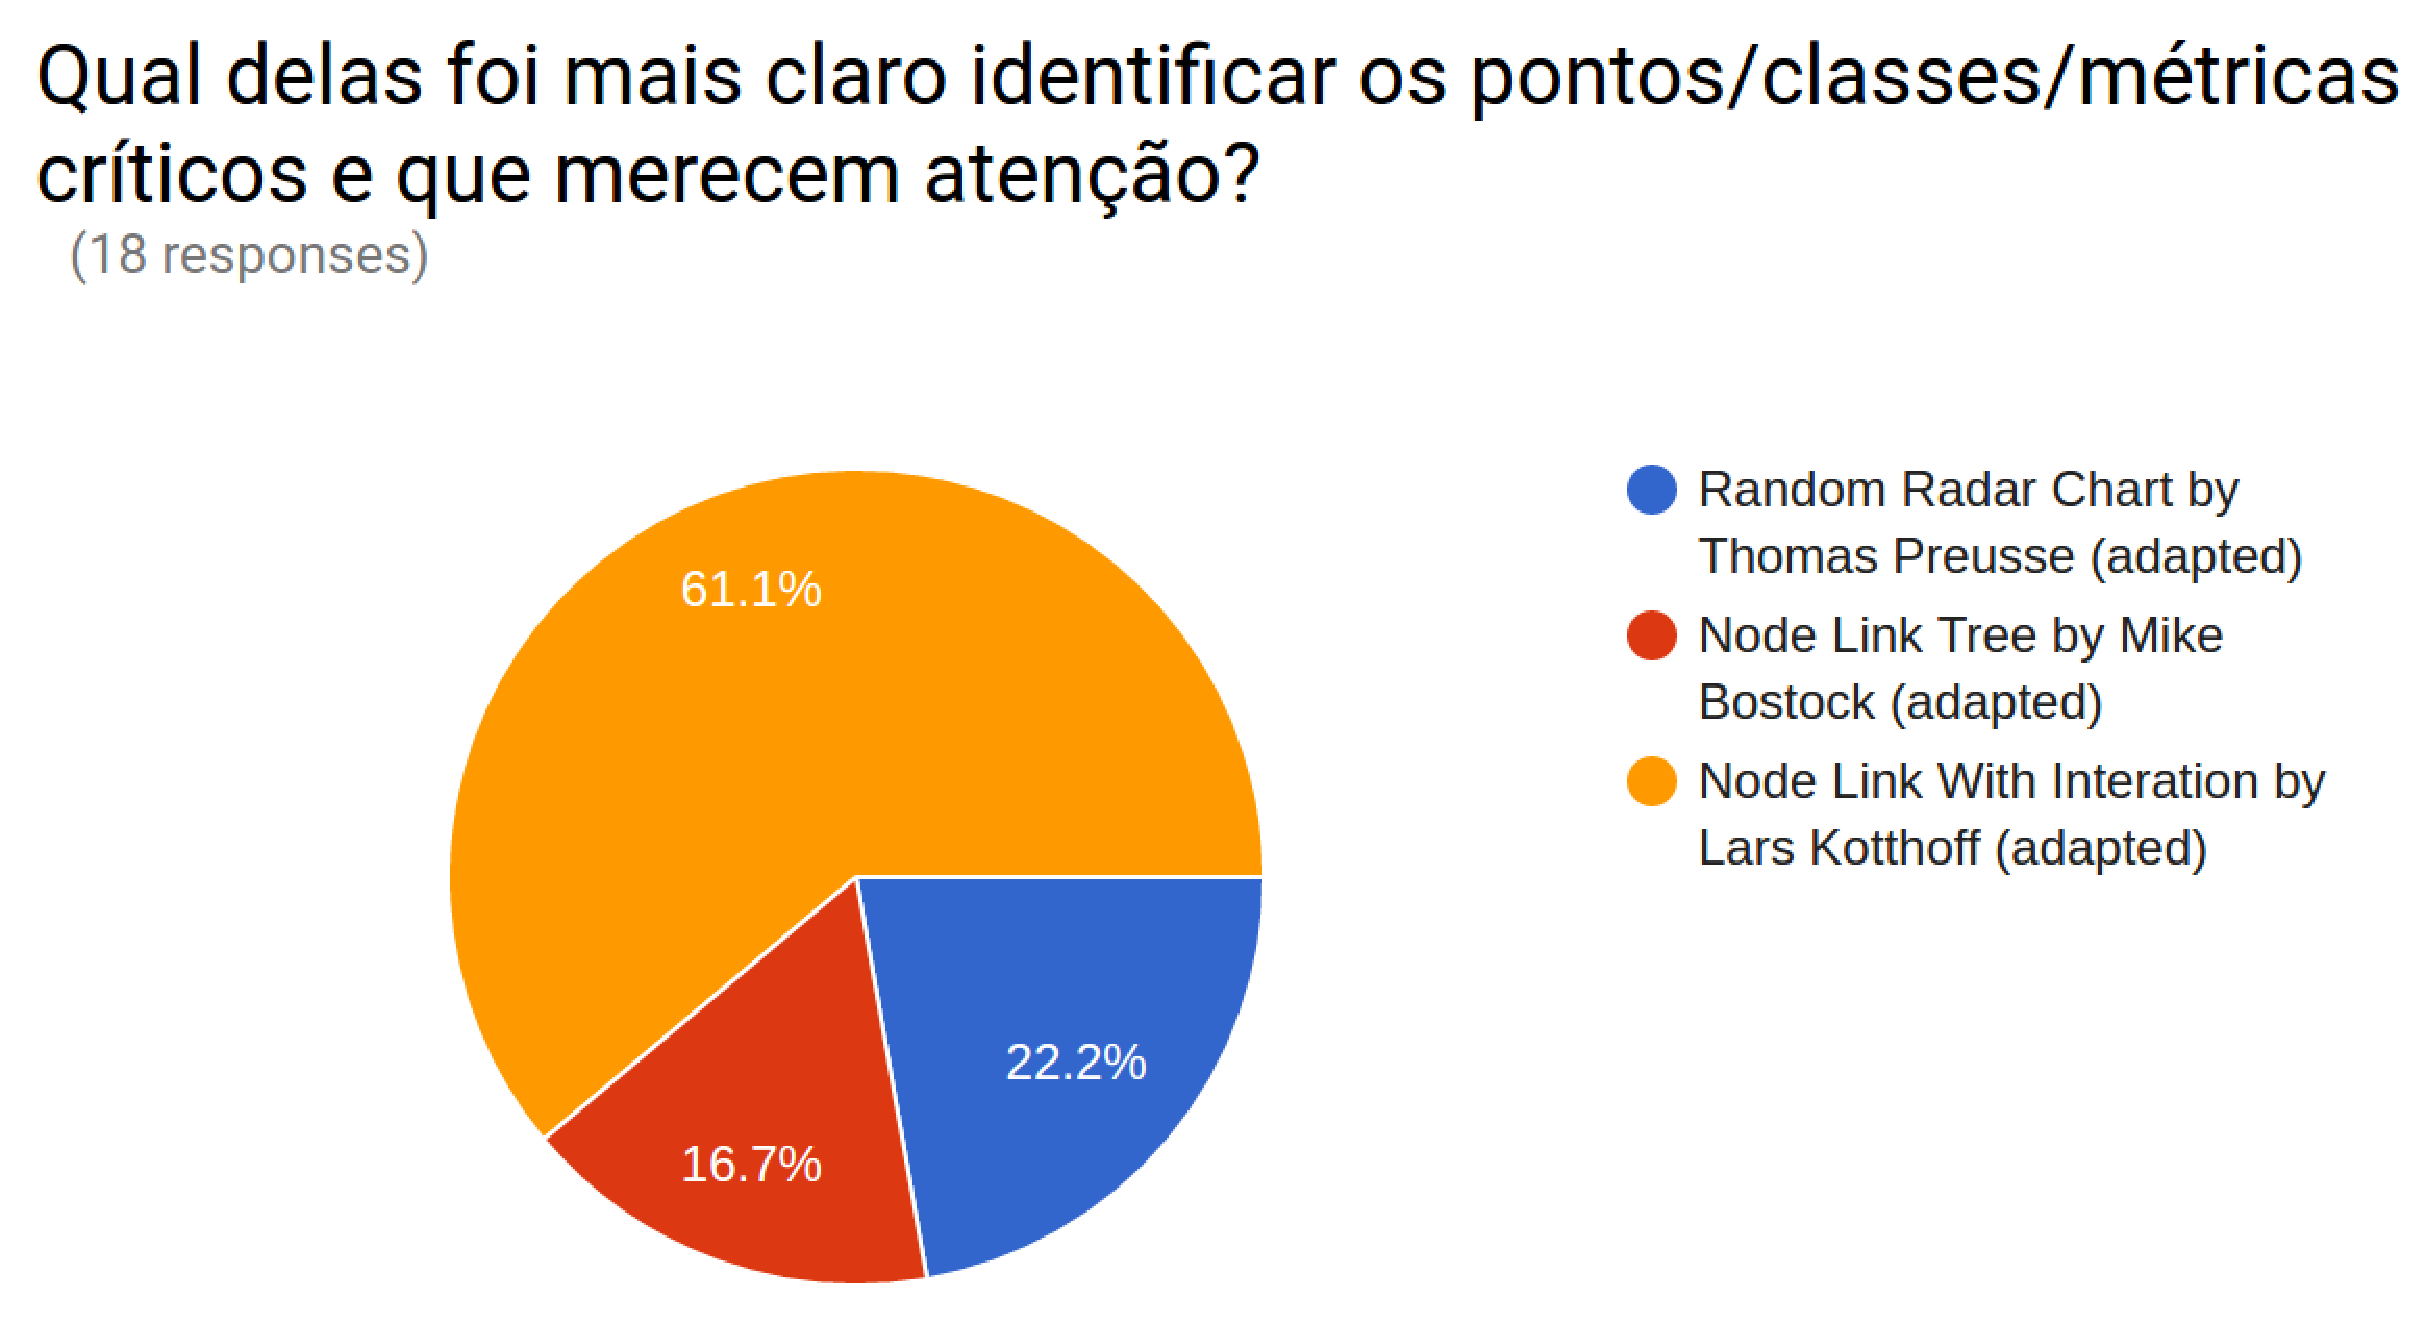
\includegraphics[keepaspectratio=true,scale=0.35]
    {figuras/res2.eps}
  \caption{Respostas para qual visualização possuia maior clareza na
  identificação dos pontos críticos}
  \label{fig:res1}
\end{figure}

Comentários, críticas e sugestões (6 respostas). Todas as respostas foram
anônimas:

\textit{"Se o método de Node With Interations, do Lars Kotthoff, começasse com
alguns nós expandidos, ele seria o melhor (na minha opinião) de longe. Como
isso não está ocorrendo, ele ainda continua melhor (na minha opinião), mas os
outros dois são mais claros para se ver o resultado final a respeito das
métricas."}

\textit{"O primeiro eu não entendi como funciona, se entendesse deve ser legal. O
segundo me deu dor de cabeça só de abrir a imagem e é ruim ficar virando a
cabeça e espremendo os olhos pra enxergar (tenho miopia)  O terceiro é legal
porque mostra tudo separadinho mas é um saco ter que clicar mil vezes pra ver
tudo."}

\textit{"Poderia colocar uma opção de visualização: Node Link With Interation
by Lars Kotthoff de vizsualizar tudo de uma vez, um expand all.}

\textit{"Para a forma de visualização do Node Link With Interation by Lars
Kotthoff (adapted) seria interessante ter um aspecto de botão para a pessoa
saber que o elemento é para ser clicado."}

\textit{"A nível de entendimento e clareza a visualização em Node Link With
Interation é a melhor, no entanto a que se apresenta de forma mais bonita é a
Node Link Tree, embora não seja tão intuitiva quanto a anterior. Além disso, a
No Link With Interation parece ter demonstrado ter capturado melhor as
necessidades, conforme a leitura das métricas, na medida em que visualmente
aponta mais valores em VERMELHO que a opção Node Link Tree. A Random Radar
Chart não evidencia valores. Não há uma escala, o que dificulta
o entendimento da gravidade da situação de uma determinada métrica."}

\textit{"Node Link Tree by Mike Bostock é a melhor, mas para ser o mais claro é
preciso trabalhar melhor com as cores usando os valores agregados de métricas.
Coloque cores em todos os nós do grafo de acordo com o grade."}


\chapter{Segundo Anexo}
\label{chap:anexoB}

As cores de fundo das colunas "Link Mezuro" e "Link CodeClimate", represetam o
resultado das análises realziadas por estas ferramentas. Se verde, a análise foi
realizada com sucesso. Se amarelo, a análise foi termiada, porém as métricas não
foram carregadas. E quando o fundo é vermelho, a análise não obteve êxito.

\begin{figure}[!htb]
	\centering
    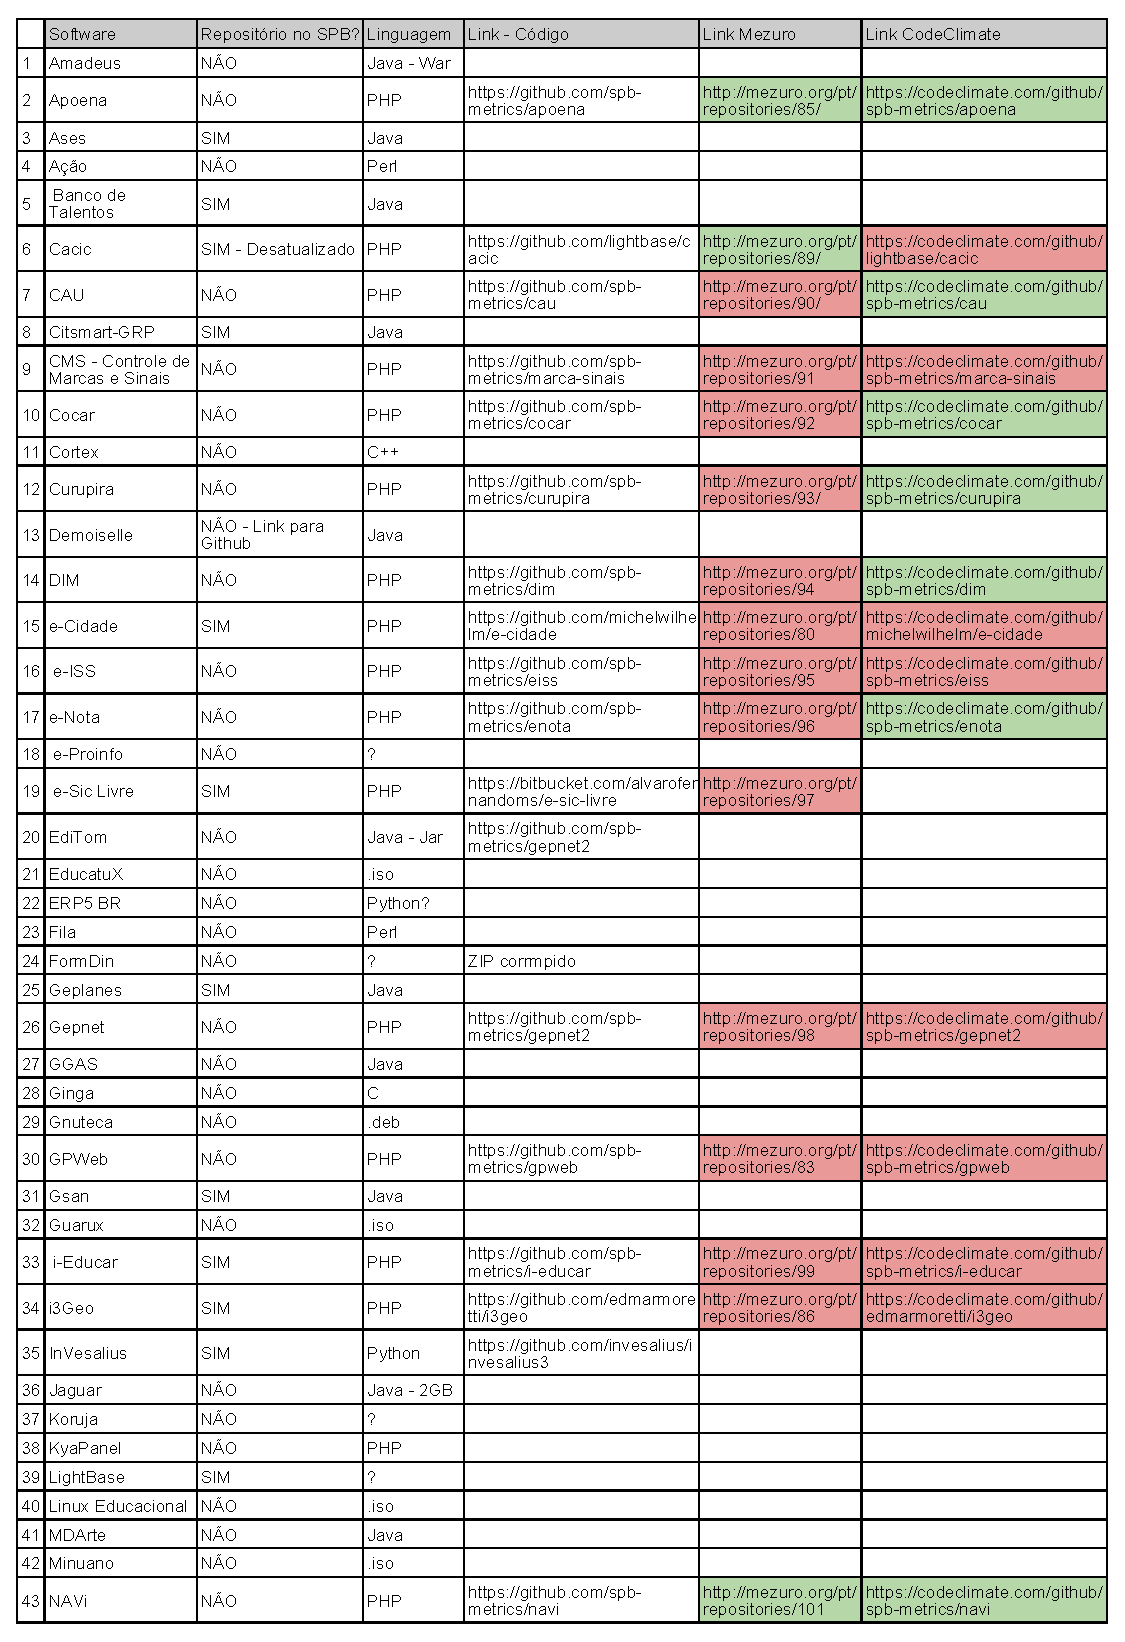
\includegraphics[keepaspectratio=true,scale=0.85]
    {tabelas/spb_1.eps}
  \caption{Categorização - Softwares SPB - Parte 1}
  \label{fig:softwares_spb_1}
\end{figure}

\begin{figure}[!htb]
	\centering
    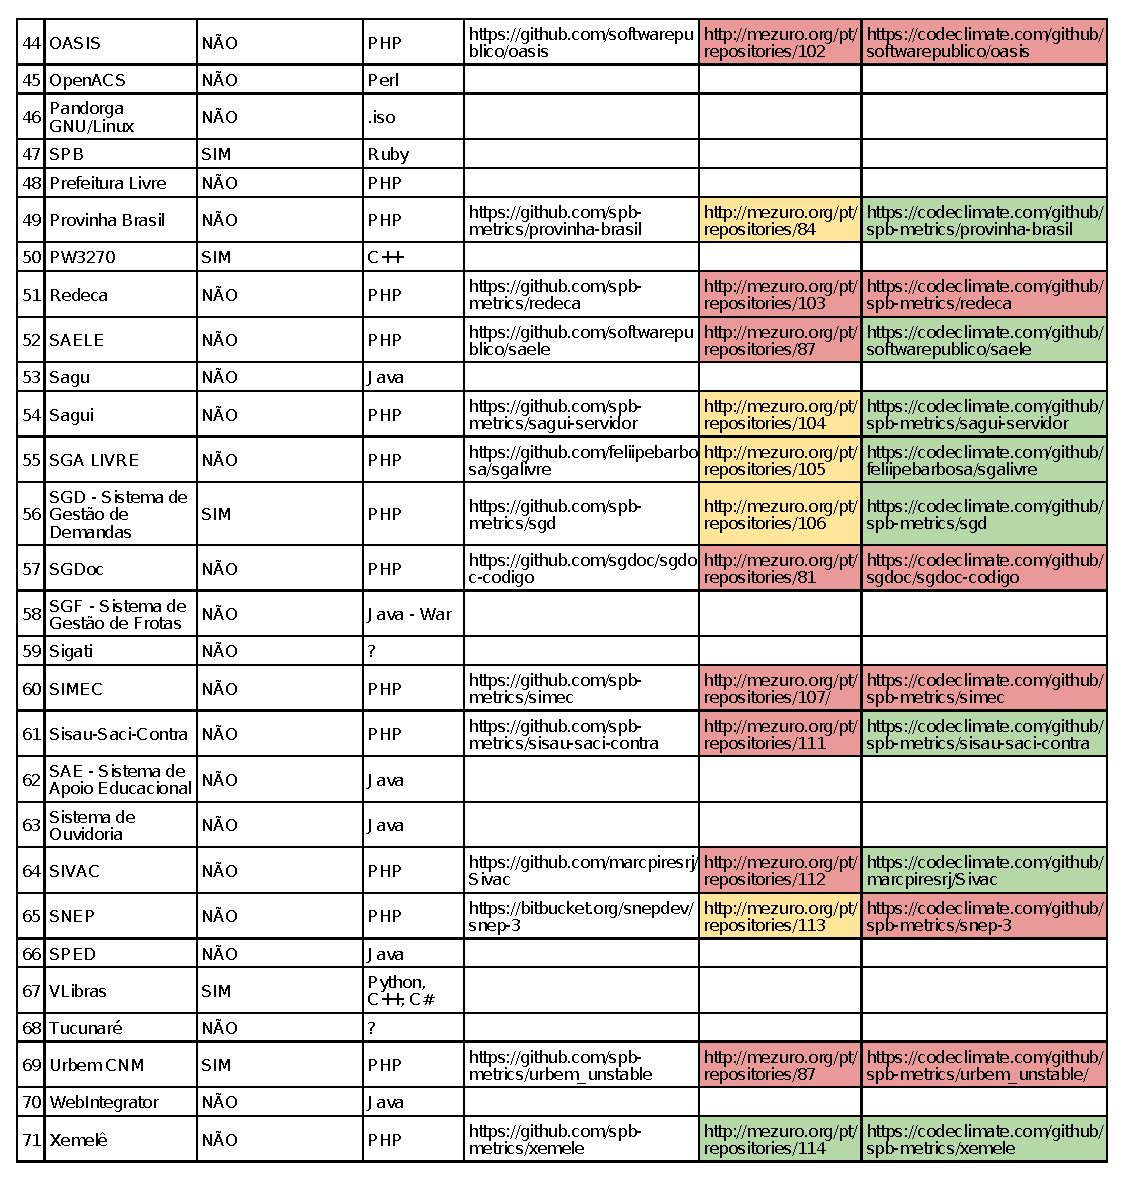
\includegraphics[keepaspectratio=true,scale=0.85]
    {tabelas/spb_2.eps}
  \caption{Categorização - Softwares SPB - Parte 2}
  \label{fig:softwares_spb_2}
\end{figure}

\end{anexosenv}

\printindex

\end{document}
